\documentclass[a4paper,14pt]{extarticle} %,twoside

%%% Проверка используемого TeX-движка %%%
\usepackage{iftex}
\newif\ifxetexorluatex   % определяем новый условный оператор (http://tex.stackexchange.com/a/47579/79756)
\ifXeTeX
    \xetexorluatextrue
\else
    \ifLuaTeX
        \xetexorluatextrue
    \else
        \xetexorluatexfalse
    \fi
\fi

%%% Поля и разметка страницы %%%
\usepackage{pdflscape}                              % Для включения альбомных страниц
\usepackage{geometry}                               % Для последующего задания полей

%%% Математические пакеты %%%
\usepackage{amsthm,amsfonts,amsmath,amssymb,amscd}  % Математические дополнения от AMS
\usepackage{mathtools}                              % Добавляет окружение multlined

%%%% Установки для размера шрифта 14 pt %%%%
%% Формирование переменных и констант для сравнения (один раз для всех подключаемых файлов)%%
%% должно располагаться до вызова пакета fontspec или polyglossia, потому что они сбивают его работу
\newlength{\curtextsize}
\newlength{\bigtextsize}
\setlength{\bigtextsize}{13.9pt}

\makeatletter
%\show\f@size                                       % неплохо для отслеживания, но вызывает стопорение процесса, если документ компилируется без команды  -interaction=nonstopmode 
\setlength{\curtextsize}{\f@size pt}
\makeatother

%%% Кодировки и шрифты %%%
\ifxetexorluatex
    \usepackage{polyglossia}                        % Поддержка многоязычности (fontspec подгружается автоматически)
\else
    \RequirePDFTeX                                  % tests for PDFTEX use and throws an error if a different engine is being used
   %%% Решение проблемы копирования текста в буфер кракозябрами
%    \input glyphtounicode.tex
%    \input glyphtounicode-cmr.tex %from pdfx package
%    \pdfgentounicode=1
    \usepackage{cmap}                               % Улучшенный поиск русских слов в полученном pdf-файле
    \defaulthyphenchar=127                          % Если стоит до fontenc, то переносы не впишутся в выделяемый текст при копировании его в буфер обмена
    \usepackage[T2A]{fontenc}                       % Поддержка русских букв
    \usepackage[utf8]{inputenc}                     % Кодировка utf8
    \usepackage[english, russian]{babel}            % Языки: русский, английский
    \IfFileExists{pscyr.sty}{\usepackage{pscyr}}{}  % Красивые русские шрифты
\fi

%%% Оформление абзацев %%%
\usepackage{indentfirst}                            % Красная строка

%%% Цвета %%%
\usepackage[dvipsnames,usenames]{color}
\usepackage{colortbl}
%\usepackage[dvipsnames, table, hyperref, cmyk]{xcolor} % Вероятно, более новый вариант, вместо предыдущих двух строк. Конвертация всех цветов в cmyk заложена как удовлетворение возможного требования типографий. Возможно конвертирование и в rgb.

%%% Таблицы %%%
\usepackage{longtable}                              % Длинные таблицы
\usepackage{multirow,makecell,array}                % Улучшенное форматирование таблиц
\usepackage{booktabs}                               % Возможность оформления таблиц в классическом книжном стиле (при правильном использовании не противоречит ГОСТ)

%%% Общее форматирование
\usepackage{soulutf8}                               % Поддержка переносоустойчивых подчёркиваний и зачёркиваний
\usepackage{icomma}                                 % Запятая в десятичных дробях


%%% Гиперссылки %%%
\usepackage{hyperref}

%%% Изображения %%%
\usepackage{graphicx}                               % Подключаем пакет работы с графикой

%%% Списки %%%
\usepackage{enumitem}

%%% Подписи %%%
\usepackage{caption}                                % Для управления подписями (рисунков и таблиц) % Может управлять номерами рисунков и таблиц с caption %Иногда может управлять заголовками в списках рисунков и таблиц
\usepackage{subcaption}                             % Работа с подрисунками и подобным

%%% Интервалы %%%
\usepackage[onehalfspacing]{setspace}               % Опция запуска пакета правит не только интервалы в обычном тексте, но и формульные

%%% Счётчики %%%
\usepackage[figure,table]{totalcount}               % Счётчик рисунков и таблиц
\usepackage{totcount}                               % Пакет создания счётчиков на основе последнего номера подсчитываемого элемента (может требовать дважды компилировать документ)
\usepackage{totpages}                               % Счётчик страниц, совместимый с hyperref (ссылается на номер последней страницы). Желательно ставить последним пакетом в преамбуле

%%% Продвинутое управление групповыми ссылками (пока только формулами) %%%
\ifxetexorluatex
    \usepackage{cleveref}                           % cleveref корректно считывает язык из настроек polyglossia
\else
    \usepackage[russian]{cleveref}                  % cleveref имеет сложности со считыванием языка из babel. Такое решение русификации вывода выбрано вместо определения в documentclass из опасности что-то лишнее передать во все остальные пакеты, включая библиографию.
\fi
\creflabelformat{equation}{#2#1#3}                  % Формат по умолчанию ставил круглые скобки вокруг каждого номера ссылки, теперь просто номера ссылок без какого-либо дополнительного оформления

\usepackage{lineno}  % Пакеты общие для диссертации и автореферата
%%% Опционально %%%
% Следующий пакет может быть полезен, если надо ужать текст, чтобы сам текст не править, но чтобы места он занимал поменьше
%\usepackage{savetrees}

% Этот пакет может быть полезен для печати текста брошюрой
%\usepackage[print]{booklet}         % Пакеты для автореферата
\usepackage{tabularx,tabulary}  %таблицы с автоматически подбирающейся шириной столбцов

% Листинги с исходным кодом программ
\usepackage{fancyvrb}
\usepackage{listings}

% Плавающие окружения. во многом лучше пакета float
\usepackage{floatrow}

% Русская традиция начертания греческих букв
%\usepackage{upgreek} % прямые греческие ради русской традиции        % Пакеты для специфических пользовательских задач

% Новые переменные, которые могут использоваться во всём проекте
\newcommand{\authorbibtitle}{Публикации автора по теме диссертации}
\newcommand{\fullbibtitle}{Список литературы} % (ГОСТ Р 7.0.11-2011, 4)
\newcommand{\snn}{ $\sqrt{ s_{NN} }$ }
\newcommand{\agev}{$A$~ГэВ}
\newcommand{\gev}{~ГэВ}
\newcommand{\ag}{Ag~+~Ag}
\newcommand{\au}{Au~+~Au}
\newcommand{\directed}{$v_1$}
\newcommand{\Ekineq}{$E_{kin}=$}  % Новые переменные, которые могут использоваться во всём проекте
%%%%%%%%%%%%%%%%%%%%%%%%%%%%%%%%%%%%%%%%%%%%%%%%%%%%%%
%%%% Файл упрощённых настроек шаблона диссертации %%%%
%%%%%%%%%%%%%%%%%%%%%%%%%%%%%%%%%%%%%%%%%%%%%%%%%%%%%%

%%%        Подключение пакетов                 %%%
\usepackage{ifthen}                 % добавляет ifthenelse
%%% Инициализирование переменных, не трогать!  %%%
\newcounter{bibliosel}
\newcounter{tabcap}
\newcounter{tablaba}
\newcounter{tabtita}
%%%%%%%%%%%%%%%%%%%%%%%%%%%%%%%%%%%%%%%%%%%%%%%%%%

%%% Область упрощённого управления оформлением %%%

%% Библиография

%% Внимание! При использовании bibtex8 необходимо удалить все
%% цитирования из  ../common/characteristic.tex 
\setcounter{bibliosel}{1}           % 0 --- встроенная реализация с загрузкой файла через движок bibtex8; 1 --- реализация пакетом biblatex через движок biber

%% Подпись таблиц
\setcounter{tabcap}{0}              % 0 --- по ГОСТ, номер таблицы и название разделены тире, выровнены по левому краю, при необходимости на нескольких строках; 1 --- подпись таблицы не по ГОСТ, на двух и более строках, дальнейшие настройки: 
%Выравнивание первой строки, с подписью и номером
\setcounter{tablaba}{2}             % 0 --- по левому краю; 1 --- по центру; 2 --- по правому краю
%Выравнивание строк с самим названием таблицы
\setcounter{tabtita}{1}             % 0 --- по левому краю; 1 --- по центру; 2 --- по правому краю

%%% Цвета гиперссылок %%%
% Latex color definitions: http://latexcolor.com/
\definecolor{linkcolor}{rgb}{0.9,0,0}
\definecolor{citecolor}{rgb}{0,0.6,0}
\definecolor{urlcolor}{rgb}{0,0,1}
%\definecolor{linkcolor}{rgb}{0,0,0} %black
%\definecolor{citecolor}{rgb}{0,0,0} %black
%\definecolor{urlcolor}{rgb}{0,0,0} %black               % Упрощённые настройки шаблона 

%%% Основные сведения %%%
\newcommand{\thesisAuthor}             % Диссертация, ФИО автора
{%
    \texorpdfstring{% \texorpdfstring takes two arguments and uses the first for (La)TeX and the second for pdf
        \todo{Мамаев Михаил Валерьевич}% так будет отображаться на титульном листе или в тексте, где будет использоваться переменная
    }{%
        Мамаев, Михаил Валерьевич% эта запись для свойств pdf-файла. В таком виде, если pdf будет обработан программами для сбора библиографических сведений, будет правильно представлена фамилия.
    }%
}
\newcommand{\thesisUdk}                % Диссертация, УДК
{\todo{xxx.xxx}}
\newcommand{\thesisTitle}              % Диссертация, название
{\texorpdfstring{\todo{\MakeUppercase{Исследование направленного потока протонов в ядро-ядерных столкновениях при энергиях $E_{kin}=$1.2 -- 4$A$~ГэВ}}}{Исследование направленного потока протонов в ядро-ядерных столкновениях при энергиях $E_{kin}=$1.2 -- 4$A$~ГэВ}}
\newcommand{\thesisSpecialtyNumber}    % Диссертация, специальность, номер
{\texorpdfstring{\todo{1.3.15}}{1.3.15}}
\newcommand{\thesisSpecialtyTitle}     % Диссертация, специальность, название
{\texorpdfstring{\todo{Физика атомного ядра и элементарных частиц. Физика Высоких энергий}}{Физика атомного ядра и элементарных частиц. Физика Высоких энергий}}
\newcommand{\thesisDegree}             % Диссертация, научная степень
{\todo{кандидата физико-математических наук}}
\newcommand{\thesisCity}               % Диссертация, город защиты
{\todo{Москва}}
\newcommand{\thesisYear}               % Диссертация, год защиты
{\todo{2024}}
\newcommand{\thesisOrganization}       % Диссертация, организация
{\todo{федеральное государственное бюджетное учреждение науки Иститут Ядерных Исследований Российской Академии Наук}}

\newcommand{\thesisInOrganization}       % Диссертация, организация в предложном падеже: Работа выполнена в ...
{\todo{федеральном государственном бюджетном учреждение науки Иституте Ядерных Исследований Российской Академии Наук}}

\newcommand{\supervisorFio}            % Научный руководитель, ФИО
{\todo{Тараненко Аркадий Владимирович}}
\newcommand{\supervisorRegalia}        % Научный руководитель, регалии
{\todo{к.ф-м. н., доцент}}

\newcommand{\opponentOneFio}           % Оппонент 1, ФИО
{\todo{Фамилия Имя Отчество}}
\newcommand{\opponentOneRegalia}       % Оппонент 1, регалии
{\todo{доктор физико-математических наук, профессор}}
\newcommand{\opponentOneJobPlace}      % Оппонент 1, место работы
{\todo{Не очень длинное название для места работы}}
\newcommand{\opponentOneJobPost}       % Оппонент 1, должность
{\todo{старший научный сотрудник}}

\newcommand{\opponentTwoFio}           % Оппонент 2, ФИО
{\todo{Фамилия Имя Отчество}}
\newcommand{\opponentTwoRegalia}       % Оппонент 2, регалии
{\todo{кандидат физико-математических наук}}
\newcommand{\opponentTwoJobPlace}      % Оппонент 2, место работы
{\todo{Основное место работы c длинным длинным длинным длинным названием}}
\newcommand{\opponentTwoJobPost}       % Оппонент 2, должность
{\todo{старший научный сотрудник}}

\newcommand{\leadingOrganizationTitle} % Ведущая организация, дополнительные строки
{\todo{Федеральное государственное бюджетное образовательное учреждение высшего профессионального образования с~длинным длинным длинным длинным названием}}

\newcommand{\defenseDate}              % Защита, дата
{\todo{DD mmmmmmmm YYYY~г.~в~XX часов}}
\newcommand{\defenseCouncilNumber}     % Защита, номер диссертационного совета
{\todo{NN}}
\newcommand{\defenseCouncilTitle}      % Защита, учреждение диссертационного совета
{\todo{Название учреждения}}
\newcommand{\defenseCouncilAddress}    % Защита, адрес учреждение диссертационного совета
{\todo{Адрес}}

\newcommand{\defenseSecretaryFio}      % Секретарь диссертационного совета, ФИО
{\todo{Фамилия Имя Отчество}}
\newcommand{\defenseSecretaryRegalia}  % Секретарь диссертационного совета, регалии
{\todo{д-р~физ.-мат. наук}}            % Для сокращений есть ГОСТы, например: ГОСТ Р 7.0.12-2011 + http://base.garant.ru/179724/#block_30000

\newcommand{\synopsisLibrary}          % Автореферат, название библиотеки
{\todo{Название библиотеки}}
\newcommand{\synopsisDate}             % Автореферат, дата рассылки
{\todo{DD mmmmmmmm YYYY года}}

\newcommand{\keywords}%                 % Ключевые слова для метаданных PDF диссертации и автореферата
{}      % Основные сведения
%%% Макет страницы %%%
% Выставляем значения полей (ГОСТ 7.0.11-2011, 5.3.7)
\geometry{a4paper,top=2cm,bottom=2cm,left=2.5cm,right=1cm}

%%% Кодировки и шрифты %%%
\ifxetexorluatex
    \setmainlanguage[babelshorthands=true]{russian}  % Язык по-умолчанию русский с поддержкой приятных команд пакета babel
    \setotherlanguage{english}                       % Дополнительный язык = английский (в американской вариации по-умолчанию)
    \ifXeTeX
        \defaultfontfeatures{Ligatures=TeX,Mapping=tex-text}
    \else
        \defaultfontfeatures{Ligatures=TeX}
    \fi
    \setmainfont{Times New Roman}
    \newfontfamily\cyrillicfont{Times New Roman}
    \setsansfont{Arial}
    \newfontfamily\cyrillicfontsf{Arial}
    \setmonofont{Courier New}
    \newfontfamily\cyrillicfonttt{Courier New}
\else
    \IfFileExists{pscyr.sty}{\renewcommand{\rmdefault}{ftm}}{}
\fi

%%% Интервалы %%%
%linespread-реализация ближе к реализации полуторного интервала в ворде.
%setspace реализация заточена под шрифты 10, 11, 12pt, под остальные кегли хуже, но всё же ближе к типографской классике. 
%\linespread{1.3}                    % Полуторный интервал (ГОСТ Р 7.0.11-2011, 5.3.6)

%%% Выравнивание и переносы %%%
\sloppy                             % Избавляемся от переполнений
\clubpenalty=10000                  % Запрещаем разрыв страницы после первой строки абзаца
\widowpenalty=10000                 % Запрещаем разрыв страницы после последней строки абзаца

%%% Подписи %%%
\captionsetup{%
singlelinecheck=off,                % Многострочные подписи, например у таблиц
skip=2pt,                           % Вертикальная отбивка между подписью и содержимым рисунка или таблицы определяется ключом
justification=centering,            % Центрирование подписей, заданных командой \caption
}

%%% Рисунки %%%
\DeclareCaptionLabelSeparator*{emdash}{~--- }             % (ГОСТ 2.105, 4.3.1)
\captionsetup[figure]{labelsep=emdash,font=onehalfspacing,position=bottom}

%%% Таблицы %%%
\ifthenelse{\equal{\thetabcap}{0}}{%
    \newcommand{\tabcapalign}{\raggedright}  % по левому краю страницы или аналога parbox
}

\ifthenelse{\equal{\thetablaba}{0} \AND \equal{\thetabcap}{1}}{%
    \newcommand{\tabcapalign}{\raggedright}  % по левому краю страницы или аналога parbox
}

\ifthenelse{\equal{\thetablaba}{1} \AND \equal{\thetabcap}{1}}{%
    \newcommand{\tabcapalign}{\centering}    % по центру страницы или аналога parbox
}

\ifthenelse{\equal{\thetablaba}{2} \AND \equal{\thetabcap}{1}}{%
    \newcommand{\tabcapalign}{\raggedleft}   % по правому краю страницы или аналога parbox
}

\ifthenelse{\equal{\thetabtita}{0} \AND \equal{\thetabcap}{1}}{%
    \newcommand{\tabtitalign}{\raggedright}  % по левому краю страницы или аналога parbox
}

\ifthenelse{\equal{\thetabtita}{1} \AND \equal{\thetabcap}{1}}{%
    \newcommand{\tabtitalign}{\centering}    % по центру страницы или аналога parbox
}

\ifthenelse{\equal{\thetabtita}{2} \AND \equal{\thetabcap}{1}}{%
    \newcommand{\tabtitalign}{\raggedleft}   % по правому краю страницы или аналога parbox
}

\DeclareCaptionFormat{tablenocaption}{\tabcapalign #1\strut}        % Наименование таблицы отсутствует
\ifthenelse{\equal{\thetabcap}{0}}{%
    \DeclareCaptionFormat{tablecaption}{\tabcapalign #1#2#3}
    \captionsetup[table]{labelsep=emdash}                       % тире как разделитель идентификатора с номером от наименования
}{%
    \DeclareCaptionFormat{tablecaption}{\tabcapalign #1#2\par%  % Идентификатор таблицы на отдельной строке
        \tabtitalign{#3}}                                       % Наименование таблицы строкой ниже
    \captionsetup[table]{labelsep=space}                        % пробельный разделитель идентификатора с номером от наименования
}
\captionsetup[table]{format=tablecaption,singlelinecheck=off,font=onehalfspacing,position=top,skip=0pt}  % многострочные наименования и прочее
\DeclareCaptionLabelFormat{continued}{Продолжение таблицы~#2}

%%% Подписи подрисунков %%%
\renewcommand{\thesubfigure}{\asbuk{subfigure}}           % Буквенные номера подрисунков
\captionsetup[subfigure]{font={normalsize},               % Шрифт подписи названий подрисунков (не отличается от основного)
    labelformat=brace,                                    % Формат обозначения подрисунка
    justification=centering,                              % Выключка подписей (форматирование), один из вариантов            
}
%\DeclareCaptionFont{font12pt}{\fontsize{12pt}{13pt}\selectfont} % объявляем шрифт 12pt для использования в подписях, тут же надо интерлиньяж объявлять, если не наследуется
%\captionsetup[subfigure]{font={font12pt}}                 % Шрифт подписи названий подрисунков (всегда 12pt)

%%% Настройки гиперссылок %%%
\ifLuaTeX
    \hypersetup{
        unicode,                % Unicode encoded PDF strings
    }
\fi

\hypersetup{
    linktocpage=true,           % ссылки с номера страницы в оглавлении, списке таблиц и списке рисунков
%    linktoc=all,                % both the section and page part are links
%    pdfpagelabels=false,        % set PDF page labels (true|false)
    plainpages=false,           % Forces page anchors to be named by the Arabic form  of the page number, rather than the formatted form
    colorlinks,                 % ссылки отображаются раскрашенным текстом, а не раскрашенным прямоугольником, вокруг текста
    linkcolor={linkcolor},      % цвет ссылок типа ref, eqref и подобных
    citecolor={citecolor},      % цвет ссылок-цитат
    urlcolor={urlcolor},        % цвет гиперссылок
%    hidelinks,                  % Hide links (removing color and border)
    pdftitle={\thesisTitle},    % Заголовок
    pdfauthor={\thesisAuthor},  % Автор
    pdfsubject={\thesisSpecialtyNumber\ \thesisSpecialtyTitle},      % Тема
%    pdfcreator={Создатель},     % Создатель, Приложение
%    pdfproducer={Производитель},% Производитель, Производитель PDF
    pdfkeywords={\keywords},    % Ключевые слова
    pdflang={ru},
}

%%% Шаблон %%%
\DeclareRobustCommand{\todo}{\textcolor{red}}       % решаем проблему превращения названия цвета в результате \MakeUppercase, http://tex.stackexchange.com/a/187930/79756 , \DeclareRobustCommand protects \todo from expanding inside \MakeUppercase
\setlength{\parindent}{2.5em}                       % Абзацный отступ. Должен быть одинаковым по всему тексту и равен пяти знакам (ГОСТ Р 7.0.11-2011, 5.3.7).

%%% Списки %%%
% Используем дефис для ненумерованных списков (ГОСТ 2.105-95, 4.1.7)
\renewcommand{\labelitemi}{\normalfont\bfseries{--}} 
\setlist{nosep,%                                    % Единый стиль для всех списков (пакет enumitem), без дополнительных интервалов.
    labelindent=\parindent,leftmargin=*%            % Каждый пункт, подпункт и перечисление записывают с абзацного отступа (ГОСТ 2.105-95, 4.1.8)
}
    % Стили общие для диссертации и автореферата
%%% Изображения %%%
\graphicspath{{images/}{Synopsis/images/}}         % Пути к изображениям

%%% Макет страницы %%%
\oddsidemargin=-13pt
\topmargin=-66pt
\headheight=12pt
\headsep=38pt
\textheight=732pt
\textwidth=484pt
\marginparsep=14pt
\marginparwidth=43pt
\footskip=14pt
\marginparpush=7pt
\hoffset=0pt
\voffset=0pt
%\paperwidth=597pt
%\paperheight=845pt
\parindent=1.5cm                  % Размер табуляции (для красной строки) в начале каждого абзаца
\renewcommand{\baselinestretch}{1.25}

\newcommand{\sfs}{\fontsize{14pt}{15pt}\selectfont}
\sfs % размер шрифта и расстояния между строками
           % Стили для автореферата
% для вертикального центрирования ячеек в tabulary
\def\zz{\ifx\[$\else\aftergroup\zzz\fi}
\def\zzz{\setbox0\lastbox
\dimen0\dimexpr\extrarowheight + \ht0-\dp0\relax
\setbox0\hbox{\raise-.5\dimen0\box0}%
\ht0=\dimexpr\ht0+\extrarowheight\relax
\dp0=\dimexpr\dp0+\extrarowheight\relax 
\box0
}



\lstdefinelanguage{Renhanced}%
{keywords={abbreviate,abline,abs,acos,acosh,action,add1,add,%
        aggregate,alias,Alias,alist,all,anova,any,aov,aperm,append,apply,%
        approx,approxfun,apropos,Arg,args,array,arrows,as,asin,asinh,%
        atan,atan2,atanh,attach,attr,attributes,autoload,autoloader,ave,%
        axis,backsolve,barplot,basename,besselI,besselJ,besselK,besselY,%
        beta,binomial,body,box,boxplot,break,browser,bug,builtins,bxp,by,%
        c,C,call,Call,case,cat,category,cbind,ceiling,character,char,%
        charmatch,check,chol,chol2inv,choose,chull,class,close,cm,codes,%
        coef,coefficients,co,col,colnames,colors,colours,commandArgs,%
        comment,complete,complex,conflicts,Conj,contents,contour,%
        contrasts,contr,control,helmert,contrib,convolve,cooks,coords,%
        distance,coplot,cor,cos,cosh,count,fields,cov,covratio,wt,CRAN,%
        create,crossprod,cummax,cummin,cumprod,cumsum,curve,cut,cycle,D,%
        data,dataentry,date,dbeta,dbinom,dcauchy,dchisq,de,debug,%
        debugger,Defunct,default,delay,delete,deltat,demo,de,density,%
        deparse,dependencies,Deprecated,deriv,description,detach,%
        dev2bitmap,dev,cur,deviance,off,prev,,dexp,df,dfbetas,dffits,%
        dgamma,dgeom,dget,dhyper,diag,diff,digamma,dim,dimnames,dir,%
        dirname,dlnorm,dlogis,dnbinom,dnchisq,dnorm,do,dotplot,double,%
        download,dpois,dput,drop,drop1,dsignrank,dt,dummy,dump,dunif,%
        duplicated,dweibull,dwilcox,dyn,edit,eff,effects,eigen,else,%
        emacs,end,environment,env,erase,eval,equal,evalq,example,exists,%
        exit,exp,expand,expression,External,extract,extractAIC,factor,%
        fail,family,fft,file,filled,find,fitted,fivenum,fix,floor,for,%
        For,formals,format,formatC,formula,Fortran,forwardsolve,frame,%
        frequency,ftable,ftable2table,function,gamma,Gamma,gammaCody,%
        gaussian,gc,gcinfo,gctorture,get,getenv,geterrmessage,getOption,%
        getwd,gl,glm,globalenv,gnome,GNOME,graphics,gray,grep,grey,grid,%
        gsub,hasTsp,hat,heat,help,hist,home,hsv,httpclient,I,identify,if,%
        ifelse,Im,image,\%in\%,index,influence,measures,inherits,install,%
        installed,integer,interaction,interactive,Internal,intersect,%
        inverse,invisible,IQR,is,jitter,kappa,kronecker,labels,lapply,%
        layout,lbeta,lchoose,lcm,legend,length,levels,lgamma,library,%
        licence,license,lines,list,lm,load,local,locator,log,log10,log1p,%
        log2,logical,loglin,lower,lowess,ls,lsfit,lsf,ls,machine,Machine,%
        mad,mahalanobis,make,link,margin,match,Math,matlines,mat,matplot,%
        matpoints,matrix,max,mean,median,memory,menu,merge,methods,min,%
        missing,Mod,mode,model,response,mosaicplot,mtext,mvfft,na,nan,%
        names,omit,nargs,nchar,ncol,NCOL,new,next,NextMethod,nextn,%
        nlevels,nlm,noquote,NotYetImplemented,NotYetUsed,nrow,NROW,null,%
        numeric,\%o\%,objects,offset,old,on,Ops,optim,optimise,optimize,%
        options,or,order,ordered,outer,package,packages,page,pairlist,%
        pairs,palette,panel,par,parent,parse,paste,path,pbeta,pbinom,%
        pcauchy,pchisq,pentagamma,persp,pexp,pf,pgamma,pgeom,phyper,pico,%
        pictex,piechart,Platform,plnorm,plogis,plot,pmatch,pmax,pmin,%
        pnbinom,pnchisq,pnorm,points,poisson,poly,polygon,polyroot,pos,%
        postscript,power,ppoints,ppois,predict,preplot,pretty,Primitive,%
        print,prmatrix,proc,prod,profile,proj,prompt,prop,provide,%
        psignrank,ps,pt,ptukey,punif,pweibull,pwilcox,q,qbeta,qbinom,%
        qcauchy,qchisq,qexp,qf,qgamma,qgeom,qhyper,qlnorm,qlogis,qnbinom,%
        qnchisq,qnorm,qpois,qqline,qqnorm,qqplot,qr,Q,qty,qy,qsignrank,%
        qt,qtukey,quantile,quasi,quit,qunif,quote,qweibull,qwilcox,%
        rainbow,range,rank,rbeta,rbind,rbinom,rcauchy,rchisq,Re,read,csv,%
        csv2,fwf,readline,socket,real,Recall,rect,reformulate,regexpr,%
        relevel,remove,rep,repeat,replace,replications,report,require,%
        resid,residuals,restart,return,rev,rexp,rf,rgamma,rgb,rgeom,R,%
        rhyper,rle,rlnorm,rlogis,rm,rnbinom,RNGkind,rnorm,round,row,%
        rownames,rowsum,rpois,rsignrank,rstandard,rstudent,rt,rug,runif,%
        rweibull,rwilcox,sample,sapply,save,scale,scan,scan,screen,sd,se,%
        search,searchpaths,segments,seq,sequence,setdiff,setequal,set,%
        setwd,show,sign,signif,sin,single,sinh,sink,solve,sort,source,%
        spline,splinefun,split,sqrt,stars,start,stat,stem,step,stop,%
        storage,strstrheight,stripplot,strsplit,structure,strwidth,sub,%
        subset,substitute,substr,substring,sum,summary,sunflowerplot,svd,%
        sweep,switch,symbol,symbols,symnum,sys,status,system,t,table,%
        tabulate,tan,tanh,tapply,tempfile,terms,terrain,tetragamma,text,%
        time,title,topo,trace,traceback,transform,tri,trigamma,trunc,try,%
        ts,tsp,typeof,unclass,undebug,undoc,union,unique,uniroot,unix,%
        unlink,unlist,unname,untrace,update,upper,url,UseMethod,var,%
        variable,vector,Version,vi,warning,warnings,weighted,weights,%
        which,while,window,write,\%x\%,x11,X11,xedit,xemacs,xinch,xor,%
        xpdrows,xy,xyinch,yinch,zapsmall,zip},%
    otherkeywords={!,!=,~,$,*,\%,\&,\%/\%,\%*\%,\%\%,<-,<<-},%
    alsoother={._$},%
    sensitive,%
    morecomment=[l]\#,%
    morestring=[d]",%
    morestring=[d]'% 2001 Robert Denham
}%

%решаем проблему с кириллицей в комментариях (в pdflatex) https://tex.stackexchange.com/a/103712/79756
\lstset{extendedchars=true,literate={Ö}{{\"O}}1
    {Ä}{{\"A}}1
    {Ü}{{\"U}}1
    {ß}{{\ss}}1
    {ü}{{\"u}}1
    {ä}{{\"a}}1
    {ö}{{\"o}}1
    {~}{{\textasciitilde}}1
    {а}{{\selectfont\char224}}1
    {б}{{\selectfont\char225}}1
    {в}{{\selectfont\char226}}1
    {г}{{\selectfont\char227}}1
    {д}{{\selectfont\char228}}1
    {е}{{\selectfont\char229}}1
    {ё}{{\"e}}1
    {ж}{{\selectfont\char230}}1
    {з}{{\selectfont\char231}}1
    {и}{{\selectfont\char232}}1
    {й}{{\selectfont\char233}}1
    {к}{{\selectfont\char234}}1
    {л}{{\selectfont\char235}}1
    {м}{{\selectfont\char236}}1
    {н}{{\selectfont\char237}}1
    {о}{{\selectfont\char238}}1
    {п}{{\selectfont\char239}}1
    {р}{{\selectfont\char240}}1
    {с}{{\selectfont\char241}}1
    {т}{{\selectfont\char242}}1
    {у}{{\selectfont\char243}}1
    {ф}{{\selectfont\char244}}1
    {х}{{\selectfont\char245}}1
    {ц}{{\selectfont\char246}}1
    {ч}{{\selectfont\char247}}1
    {ш}{{\selectfont\char248}}1
    {щ}{{\selectfont\char249}}1
    {ъ}{{\selectfont\char250}}1
    {ы}{{\selectfont\char251}}1
    {ь}{{\selectfont\char252}}1
    {э}{{\selectfont\char253}}1
    {ю}{{\selectfont\char254}}1
    {я}{{\selectfont\char255}}1
    {А}{{\selectfont\char192}}1
    {Б}{{\selectfont\char193}}1
    {В}{{\selectfont\char194}}1
    {Г}{{\selectfont\char195}}1
    {Д}{{\selectfont\char196}}1
    {Е}{{\selectfont\char197}}1
    {Ё}{{\"E}}1
    {Ж}{{\selectfont\char198}}1
    {З}{{\selectfont\char199}}1
    {И}{{\selectfont\char200}}1
    {Й}{{\selectfont\char201}}1
    {К}{{\selectfont\char202}}1
    {Л}{{\selectfont\char203}}1
    {М}{{\selectfont\char204}}1
    {Н}{{\selectfont\char205}}1
    {О}{{\selectfont\char206}}1
    {П}{{\selectfont\char207}}1
    {Р}{{\selectfont\char208}}1
    {С}{{\selectfont\char209}}1
    {Т}{{\selectfont\char210}}1
    {У}{{\selectfont\char211}}1
    {Ф}{{\selectfont\char212}}1
    {Х}{{\selectfont\char213}}1
    {Ц}{{\selectfont\char214}}1
    {Ч}{{\selectfont\char215}}1
    {Ш}{{\selectfont\char216}}1
    {Щ}{{\selectfont\char217}}1
    {Ъ}{{\selectfont\char218}}1
    {Ы}{{\selectfont\char219}}1
    {Ь}{{\selectfont\char220}}1
    {Э}{{\selectfont\char221}}1
    {Ю}{{\selectfont\char222}}1
    {Я}{{\selectfont\char223}}1
    {і}{{\selectfont\char105}}1
    {ї}{{\selectfont\char168}}1
    {є}{{\selectfont\char185}}1
    {ґ}{{\selectfont\char160}}1
    {І}{{\selectfont\char73}}1
    {Ї}{{\selectfont\char136}}1
    {Є}{{\selectfont\char153}}1
    {Ґ}{{\selectfont\char128}}1
}

% Ширина текста минус ширина надписи 999
\newlength{\twless}
\newlength{\lmarg}
\setlength{\lmarg}{\widthof{999}}   % ширина надписи 999
\setlength{\twless}{\textwidth-\lmarg}


\lstset{ %
%    language=R,                     %  Язык указать здесь, если во всех листингах преимущественно один язык, в результате часть настроек может пойти только для этого языка
    numbers=left,                   % where to put the line-numbers
    numberstyle=\fontsize{12pt}{14pt}\selectfont\color{Gray},  % the style that is used for the line-numbers
    firstnumber=2,                  % в этой и следующей строках задаётся поведение нумерации 5, 10, 15...
    stepnumber=5,                   % the step between two line-numbers. If it's 1, each line will be numbered
    numbersep=5pt,                  % how far the line-numbers are from the code
    backgroundcolor=\color{white},  % choose the background color. You must add \usepackage{color}
    showspaces=false,               % show spaces adding particular underscores
    showstringspaces=false,         % underline spaces within strings
    showtabs=false,                 % show tabs within strings adding particular underscores
    frame=leftline,                 % adds a frame of different types around the code
    rulecolor=\color{black},        % if not set, the frame-color may be changed on line-breaks within not-black text (e.g. commens (green here))
    tabsize=2,                      % sets default tabsize to 2 spaces
    captionpos=t,                   % sets the caption-position to top
    breaklines=true,                % sets automatic line breaking
    breakatwhitespace=false,        % sets if automatic breaks should only happen at whitespace
%    title=\lstname,                 % show the filename of files included with \lstinputlisting;
    % also try caption instead of title
    basicstyle=\fontsize{12pt}{14pt}\selectfont\ttfamily,% the size of the fonts that are used for the code
%    keywordstyle=\color{blue},      % keyword style
    commentstyle=\color{ForestGreen}\emph,% comment style
    stringstyle=\color{Mahogany},   % string literal style
    escapeinside={\%*}{*)},         % if you want to add a comment within your code
    morekeywords={*,...},           % if you want to add more keywords to the set
    inputencoding=utf8,             % кодировка кода
    xleftmargin={\lmarg},           % Чтобы весь код и полоска с номерами строк была смещена влево, так чтобы цифры не вылезали за пределы текста слева
} 

%http://tex.stackexchange.com/questions/26872/smaller-frame-with-listings
% Окружение, чтобы листинг был компактнее обведен рамкой, если она задается, а не на всю ширину текста
\makeatletter
\newenvironment{SmallListing}[1][]
{\lstset{#1}\VerbatimEnvironment\begin{VerbatimOut}{VerbEnv.tmp}}
{\end{VerbatimOut}\settowidth\@tempdima{%
        \lstinputlisting{VerbEnv.tmp}}
    \minipage{\@tempdima}\lstinputlisting{VerbEnv.tmp}\endminipage}    
\makeatother


\DefineVerbatimEnvironment% с шрифтом 12 пт
{Verb}{Verbatim}
{fontsize=\fontsize{12pt}{14pt}\selectfont}

\RawFloats[figure,table]            % Отмена установок пакета floatrow для всех флотов (плавающих окружений) выбранных типов или подтипов. А то будто мы зря задавали настройки подписей рисунков и таблиц. 

\DeclareNewFloatType{ListingEnv}{
    placement=htb,
    within=chapter,
    fileext=lol,
    name=Листинг,
}

\captionsetup[ListingEnv]{
    format=tablecaption,
    labelsep=space,                 % Точка после номера листинга задается значением period
    singlelinecheck=off,
    font=onehalfspacing,
    position=top,
}


\floatsetup[ListingEnv]{
    style=plaintop,
    captionskip=4pt,
}

\captionsetup[lstlisting]{
    format=tablecaption,
    labelsep=space,                 % Точка после номера листинга задается значением period
    singlelinecheck=off,
    font=onehalfspacing,
    position=top,
}

\renewcommand{\lstlistingname}{Листинг}

%Общие счётчики окружений листингов
%http://tex.stackexchange.com/questions/145546/how-to-make-figure-and-listing-share-their-counter
% Если смешивать плавающие и не плавающие окружения, то могут быть проблемы с нумерацией
\makeatletter
\AtBeginDocument{%
    \let\c@ListingEnv\c@lstlisting
    \let\theListingEnv\thelstlisting
    \let\ftype@lstlisting\ftype@ListingEnv % give the floats the same precedence
}
\makeatother

% значок С++ — используйте команду \cpp
\newcommand{\cpp}{%
    C\nolinebreak\hspace{-.05em}%
    \raisebox{.2ex}{+}\nolinebreak\hspace{-.10em}%
    \raisebox{.2ex}{+}%
}


%%% Русская традиция начертания математических знаков
%\renewcommand{\le}{\ensuremath{\leqslant}}
%\renewcommand{\leq}{\ensuremath{\leqslant}}
%\renewcommand{\ge}{\ensuremath{\geqslant}}
%\renewcommand{\geq}{\ensuremath{\geqslant}}
%\renewcommand{\emptyset}{\varnothing}

%%% Русская традиция начертания греческих букв (греческие буквы вертикальные, через пакет upgreek)
%\renewcommand{\epsilon}{\ensuremath{\upvarepsilon}}   %  русская традиция записи
%\renewcommand{\phi}{\ensuremath{\upvarphi}}
%%\renewcommand{\kappa}{\ensuremath{\varkappa}}
%\renewcommand{\alpha}{\upalpha}
%\renewcommand{\beta}{\upbeta}
%\renewcommand{\gamma}{\upgamma}
%\renewcommand{\delta}{\updelta}
%\renewcommand{\varepsilon}{\upvarepsilon}
%\renewcommand{\zeta}{\upzeta}
%\renewcommand{\eta}{\upeta}
%\renewcommand{\theta}{\uptheta}
%\renewcommand{\vartheta}{\upvartheta}
%\renewcommand{\iota}{\upiota}
%\renewcommand{\kappa}{\upkappa}
%\renewcommand{\lambda}{\uplambda}
%\renewcommand{\mu}{\upmu}
%\renewcommand{\nu}{\upnu}
%\renewcommand{\xi}{\upxi}
%\renewcommand{\pi}{\uppi}
%\renewcommand{\varpi}{\upvarpi}
%\renewcommand{\rho}{\uprho}
%%\renewcommand{\varrho}{\upvarrho}
%\renewcommand{\sigma}{\upsigma}
%%\renewcommand{\varsigma}{\upvarsigma}
%\renewcommand{\tau}{\uptau}
%\renewcommand{\upsilon}{\upupsilon}
%\renewcommand{\varphi}{\upvarphi}
%\renewcommand{\chi}{\upchi}
%\renewcommand{\psi}{\uppsi}
%\renewcommand{\omega}{\upomega}
          % Стили для специфических пользовательских задач
%%% Библиография. Общие настройки для двух способов её подключения %%%


%%% Выбор реализации %%%
\ifthenelse{\equal{\thebibliosel}{0}}{%
    %%% Реализация библиографии встроенными средствами посредством движка bibtex8 %%%

%%% Пакеты %%%
\usepackage{cite}                                   % Красивые ссылки на литературу


%%% Стили %%%
\bibliographystyle{BibTeX-Styles/utf8gost71u}    % Оформляем библиографию по ГОСТ 7.1 (ГОСТ Р 7.0.11-2011, 5.6.7)

\makeatletter
\renewcommand{\@biblabel}[1]{#1.}   % Заменяем библиографию с квадратных скобок на точку
\makeatother
%% Управление отступами между записями
%% требует etoolbox 
%% http://tex.stackexchange.com/a/105642
%\patchcmd\thebibliography
% {\labelsep}
% {\labelsep\itemsep=5pt\parsep=0pt\relax}
% {}
% {\typeout{Couldn't patch the command}}

%%% Список литературы с красной строки (без висячего отступа) %%%
%\patchcmd{\thebibliography} %может потребовать включения пакета etoolbox
%  {\advance\leftmargin\labelsep}
%  {\leftmargin=0pt%
%   \setlength{\labelsep}{\widthof{\ }}% Управляет длиной отступа после точки
%   \itemindent=\parindent%
%   \addtolength{\itemindent}{\labelwidth}% Сдвигаем правее на величину номера с точкой
%   \advance\itemindent\labelsep%
%  }
%  {}{}

%%% Цитирование %%%
\renewcommand\citepunct{;\penalty\citepunctpenalty%
    \hskip.13emplus.1emminus.1em\relax}                % Разделение ; при перечислении ссылок (ГОСТ Р 7.0.5-2008)


%%% Создание команд для вывода списка литературы %%%
\newcommand*{\insertbibliofull}{
\bibliography{biblio/othercites,biblio/authorpapersVAK,biblio/authorpapers,biblio/authorconferences}         % Подключаем BibTeX-базы % После запятых не должно быть лишних пробелов — он "думает", что это тоже имя пути
}

\newcommand*{\insertbiblioauthor}{
\bibliography{biblio/authorpapersVAK,biblio/authorpapers,biblio/authorconferences}         % Подключаем BibTeX-базы % После запятых не должно быть лишних пробелов — он "думает", что это тоже имя пути
}

\newcommand*{\insertbiblioother}{
\bibliography{biblio/othercites}         % Подключаем BibTeX-базы
}


%% Счётчик использованных ссылок на литературу, обрабатывающий с учётом неоднократных ссылок
%% Требуется дважды компилировать, поскольку ему нужно считать актуальный внешний файл со списком литературы
\newtotcounter{citenum}
\def\oldcite{}
\let\oldcite=\bibcite
\def\bibcite{\stepcounter{citenum}\oldcite}
  % Встроенная реализация с загрузкой файла через движок bibtex8
}{
    %%% Реализация библиографии пакетами biblatex и biblatex-gost с использованием движка biber %%%

%\usepackage{csquotes} % biblatex рекомендует его подключать. Пакет для оформления сложных блоков цитирования.

%%% Загрузка пакета с основными настройками %%%
\usepackage[%
backend=biber,% движок
bibencoding=utf8,% кодировка bib файла
sorting=none,% настройка сортировки списка литературы
style=gost-numeric,% стиль цитирования и библиографии (по ГОСТ)
language=autobib,% получение языка из babel/polyglossia, default: autobib % если ставить autocite или auto, то цитаты в тексте с указанием страницы, получат указание страницы на языке оригинала
autolang=other,% многоязычная библиография
clearlang=true,% внутренний сброс поля language, если он совпадает с языком из babel/polyglossia
defernumbers=true,% нумерация проставляется после двух компиляций, зато позволяет выцеплять библиографию по ключевым словам и нумеровать не из большего списка
sortcites=true,% сортировать номера затекстовых ссылок при цитировании (если в квадратных скобках несколько ссылок, то отображаться будут отсортированно, а не абы как)
doi=false,% Показывать или нет ссылки на DOI
%isbn=false,% Показывать или нет ISBN
]{biblatex}


%http://tex.stackexchange.com/a/141831/79756
%There is a way to automatically map the language field to the langid field. The following lines in the preamble should be enough to do that.
%This command will copy the language field into the langid field and will then delete the contents of the language field. The language field will only be deleted if it was successfully copied into the langid field.
\DeclareSourcemap{ %модификация bib файла перед тем, как им займётся biblatex 
    \maps{
        \map{% перекидываем значения полей language в поля langid, которыми пользуется biblatex
            \step[fieldsource=language, fieldset=langid, origfieldval, final]
            \step[fieldset=language, null]
        }
        \map{% перекидываем значения полей numpages в поля pagetotal, которыми пользуется biblatex
            \step[fieldsource=numpages, fieldset=pagetotal, origfieldval, final]
            \step[fieldset=pagestotal, null]
        }
        \map{% если в поле medium написано "Электронный ресурс", то устанавливаем поле media. которым пользуется biblatex в значение eresource
            \step[fieldsource=medium,
            match=\regexp{Электронный\s+ресурс},
            final]
            \step[fieldset=media, fieldvalue=eresource]
        }
        \map[overwrite]{% стираем значения всех полей issn
            \step[fieldset=issn, null]
        }
        \map[overwrite]{% стираем значения всех полей abstract, поскольку ими не пользуемся, а там бывают "неприятные" латеху символы
            \step[fieldsource=abstract]
            \step[fieldset=abstract,null]
        }
        \map[overwrite]{ % переделка формата записи даты
            \step[fieldsource=urldate,
            match=\regexp{([0-9]{2})\.([0-9]{2})\.([0-9]{4})},
            replace={$3-$2-$1$4}, % $4 вставлен исключительно ради нормальной работы программ подсветки синтаксиса, которые некорректно обрабатывают $ в таких конструкциях
            final]
        }
        \map[overwrite]{ % добавляем ключевые слова, чтобы различать источники
            \perdatasource{biblio/othercites.bib}
            \step[fieldset=keywords, fieldvalue={biblioother,bibliofull}]
        }
        \map[overwrite]{ % добавляем ключевые слова, чтобы различать источники
            \perdatasource{biblio/authorpapersVAK.bib}
            \step[fieldset=keywords, fieldvalue={biblioauthorvak,biblioauthor,bibliofull}]
        }
        \map[overwrite]{ % добавляем ключевые слова, чтобы различать источники
            \perdatasource{biblio/authorpapers.bib}
            \step[fieldset=keywords, fieldvalue={biblioauthornotvak,biblioauthor,bibliofull}]
        }
        \map[overwrite]{ % добавляем ключевые слова, чтобы различать источники
            \perdatasource{biblio/authorconferences.bib}
            \step[fieldset=keywords, fieldvalue={biblioauthorconf,biblioauthor,bibliofull}]
        }
%        \map[overwrite]{% стираем значения всех полей series
%            \step[fieldset=series, null]
%        }
        \map[overwrite]{% перекидываем значения полей howpublished в поля organization для типа online
            \step[typesource=online, fieldsource=howpublished, fieldset=organization, origfieldval, final]
            \step[fieldset=howpublished, null]
        }
        % Так отключаем [Электронный ресурс]
%        \map[overwrite]{% стираем значения всех полей media=eresource
%            \step[fieldsource=media,
%            match={eresource},
%            final]
%            \step[fieldset=media, null]
%        }
    }
}

%%% Правка записей типа thesis, чтобы дважды не писался автор
%\DeclareBibliographyDriver{thesis}{%
%  \usebibmacro{bibindex}%
%  \usebibmacro{begentry}%
%  \usebibmacro{heading}%
%  \newunit
%  \usebibmacro{author}%
%  \setunit*{\labelnamepunct}%
%  \usebibmacro{thesistitle}%
%  \setunit{\respdelim}%
%  %\printnames[last-first:full]{author}%Вот эту строчку нужно убрать, чтобы автор диссертации не дублировался
%  \newunit\newblock
%  \printlist[semicolondelim]{specdata}%
%  \newunit
%  \usebibmacro{institution+location+date}%
%  \newunit\newblock
%  \usebibmacro{chapter+pages}%
%  \newunit
%  \printfield{pagetotal}%
%  \newunit\newblock
%  \usebibmacro{doi+eprint+url+note}%
%  \newunit\newblock
%  \usebibmacro{addendum+pubstate}%
%  \setunit{\bibpagerefpunct}\newblock
%  \usebibmacro{pageref}%
%  \newunit\newblock
%  \usebibmacro{related:init}%
%  \usebibmacro{related}%
%  \usebibmacro{finentry}}


%\newbibmacro{string+doi}[1]{% новая макрокоманда на простановку ссылки на doi
%    \iffieldundef{doi}{#1}{\href{http://dx.doi.org/\thefield{doi}}{#1}}}
%
%\renewcommand*{\mkgostheading}[1]{\usebibmacro{string+doi}{#1}} % ссылка на doi с авторов. стоящих впереди записи
%\renewcommand*{\mkgostheading}[1]{#1} % только лишь убираем курсив с авторов
%\DeclareFieldFormat{title}{\usebibmacro{string+doi}{#1}} % ссылка на doi с названия работы
%\DeclareFieldFormat{journaltitle}{\usebibmacro{string+doi}{#1}} % ссылка на doi с названия журнала
% Убрать тире из разделителей элементов в библиографии:
%\renewcommand*{\newblockpunct}{%
%    \addperiod\space\bibsentence}%block punct.,\bibsentence is for vol,etc.

%%% Возвращаем запись «Режим доступа» %%%
%\DefineBibliographyStrings{english}{%
%    urlfrom = {Mode of access}
%}
%\DeclareFieldFormat{url}{\bibstring{urlfrom}\addcolon\space\url{#1}}

%%% Set low penalties for breaks at uppercase letters and lowercase letters
%\setcounter{biburllcpenalty}{500} %управляет разрывами ссылок после маленьких букв RTFM biburllcpenalty
%\setcounter{biburlucpenalty}{3000} %управляет разрывами ссылок после больших букв, RTFM biburlucpenalty

%%% Список литературы с красной строки (без висячего отступа) %%%
%\defbibenvironment{bibliography} % переопределяем окружение библиографии из gost-numeric.bbx пакета biblatex-gost
%  {\list
%     {\printtext[labelnumberwidth]{%
%	\printfield{prefixnumber}%
%	\printfield{labelnumber}}}
%     {%
%      \setlength{\labelwidth}{\labelnumberwidth}%
%      \setlength{\leftmargin}{0pt}% default is \labelwidth
%      \setlength{\labelsep}{\widthof{\ }}% Управляет длиной отступа после точки % default is \biblabelsep
%      \setlength{\itemsep}{\bibitemsep}% Управление дополнительным вертикальным разрывом между записями. \bibitemsep по умолчанию соответствует \itemsep списков в документе.
%      \setlength{\itemindent}{\bibhang}% Пользуемся тем, что \bibhang по умолчанию принимает значение \parindent (абзацного отступа), который переназначен в styles.tex
%      \addtolength{\itemindent}{\labelwidth}% Сдвигаем правее на величину номера с точкой
%      \addtolength{\itemindent}{\labelsep}% Сдвигаем ещё правее на отступ после точки
%      \setlength{\parsep}{\bibparsep}%
%     }%
%      \renewcommand*{\makelabel}[1]{\hss##1}%
%  }
%  {\endlist}
%  {\item}

%%% Подключение файлов bib %%%
\addbibresource{biblio/othercites.bib}
\addbibresource{biblio/authorpapersVAK.bib}
\addbibresource{biblio/authorpapers.bib}
\addbibresource{biblio/authorconferences.bib}


%% Счётчик использованных ссылок на литературу, обрабатывающий с учётом неоднократных ссылок
%http://tex.stackexchange.com/a/66851/79756
%\newcounter{citenum}
\newtotcounter{citenum}
\makeatletter
\defbibenvironment{counter} %Env of bibliography
  {\setcounter{citenum}{0}%
  \renewcommand{\blx@driver}[1]{}%
  } %what is doing at the beginining of bibliography. In your case it's : a. Reset counter b. Say to print nothing when a entry is tested.
  {} %Здесь то, что будет выводиться командой \printbibliography. \thecitenum сюда писать не надо
  {\stepcounter{citenum}} %What is printing / executed at each entry.
\makeatother
\defbibheading{counter}{}



\newtotcounter{citeauthorvak}
\makeatletter
\defbibenvironment{countauthorvak} %Env of bibliography
{\setcounter{citeauthorvak}{0}%
    \renewcommand{\blx@driver}[1]{}%
} %what is doing at the beginining of bibliography. In your case it's : a. Reset counter b. Say to print nothing when a entry is tested.
{} %Здесь то, что будет выводиться командой \printbibliography. Обойдёмся без \theciteauthorvak в нашей реализации
{\stepcounter{citeauthorvak}} %What is printing / executed at each entry.
\makeatother
\defbibheading{countauthorvak}{}

\newtotcounter{citeauthornotvak}
\makeatletter
\defbibenvironment{countauthornotvak} %Env of bibliography
{\setcounter{citeauthornotvak}{0}%
    \renewcommand{\blx@driver}[1]{}%
} %what is doing at the beginining of bibliography. In your case it's : a. Reset counter b. Say to print nothing when a entry is tested.
{} %Здесь то, что будет выводиться командой \printbibliography. Обойдёмся без \theciteauthornotvak в нашей реализации
{\stepcounter{citeauthornotvak}} %What is printing / executed at each entry.
\makeatother
\defbibheading{countauthornotvak}{}

\newtotcounter{citeauthorconf}
\makeatletter
\defbibenvironment{countauthorconf} %Env of bibliography
{\setcounter{citeauthorconf}{0}%
    \renewcommand{\blx@driver}[1]{}%
} %what is doing at the beginining of bibliography. In your case it's : a. Reset counter b. Say to print nothing when a entry is tested.
{} %Здесь то, что будет выводиться командой \printbibliography. Обойдёмся без \theciteauthorconf в нашей реализации
{\stepcounter{citeauthorconf}} %What is printing / executed at each entry.
\makeatother
\defbibheading{countauthorconf}{}

\newtotcounter{citeauthor}
\makeatletter
\defbibenvironment{countauthor} %Env of bibliography
{\setcounter{citeauthor}{0}%
    \renewcommand{\blx@driver}[1]{}%
} %what is doing at the beginining of bibliography. In your case it's : a. Reset counter b. Say to print nothing when a entry is tested.
{} %Здесь то, что будет выводиться командой \printbibliography. Обойдёмся без \theciteauthor в нашей реализации
{\stepcounter{citeauthor}} %What is printing / executed at each entry.
\makeatother
\defbibheading{countauthor}{}

%%% Создание команд для вывода списка литературы %%%
\newcommand*{\insertbibliofull}{
\printbibliography[keyword=bibliofull,section=0]
\printbibliography[heading=counter,env=counter,keyword=bibliofull,section=0]
}

\newcommand*{\insertbiblioauthor}{
\printbibliography[keyword=biblioauthor,section=1,title=\authorbibtitle]
\printbibliography[heading=counter,env=counter,keyword=biblioauthor,section=1]
}

\newcommand*{\insertbiblioother}{
\printbibliography[keyword=biblioother]
\printbibliography[heading=counter,env=counter,keyword=biblioother]
}    % Реализация пакетом biblatex через движок biber
}
% Настройки библиографии из внешнего файла (там же выбор: встроенная или на основе biblatex)

\begin{document}

\thispagestyle{empty}

\vspace{0pt plus1fill} %число перед fill = кратность относительно некоторого расстояния fill, кусками которого заполнены пустые места
\begin{flushright}
  \large{На правах рукописи}
  
  
\includegraphics[height=1.5cm]{mamaev_signature.jpg} 
\end{flushright}

\vspace{0pt plus3fill} %число перед fill = кратность относительно некоторого расстояния fill, кусками которого заполнены пустые места
\begin{center}
\textbf {\large \thesisAuthor}
\end{center}

\vspace{0pt plus3fill} %число перед fill = кратность относительно некоторого расстояния fill, кусками которого заполнены пустые места
\begin{center}
\textbf {\Large \thesisTitle}

\vspace{0pt plus3fill} %число перед fill = кратность относительно некоторого расстояния fill, кусками которого заполнены пустые места
{\large Специальность \thesisSpecialtyNumber\ "---\par <<\thesisSpecialtyTitle>>}

\vspace{0pt plus1.5fill} %число перед fill = кратность относительно некоторого расстояния fill, кусками которого заполнены пустые места
\Large{Автореферат}\par
\large{диссертации на соискание учёной степени\par \thesisDegree}
\end{center}

\vspace{0pt plus4fill} %число перед fill = кратность относительно некоторого расстояния fill, кусками которого заполнены пустые места
\begin{center}
{\large{\thesisCity\ "--- \thesisYear}}
\end{center}

\newpage
% оборотная сторона обложки
\thispagestyle{empty}
\noindent Работа выполнена в \thesisInOrganization

\par\bigskip
%\begin{table}[h] % считается не очень правильным использовать окружение table, не задавая caption
    \noindent%
    \begin{tabular}{@{}lp{11cm}}
        \sfs Научный руководитель: & \sfs \supervisorRegalia \par
                                      \textbf{\supervisorFio}
        \vspace{4mm} \\
        {\sfs Официальные оппоненты:} &
        {\sfs \textbf{\opponentOneFio,}\par
                  \opponentOneRegalia,\par
                  \opponentOneJobPlace,\par
                  \opponentOneJobPost\par \vspace{3mm}
                  \textbf{\opponentTwoFio,}\par \vspace{1mm}
                  \opponentTwoRegalia,\par
                  \opponentTwoJobPlace,\par
                  \opponentTwoJobPost
        }
        \vspace{4mm} \\
        {\sfs Ведущая организация:} & {\sfs \leadingOrganizationTitle }
    \end{tabular}  
%\end{table}
\par\bigskip

\noindent Защита состоится \defenseDate~на~заседании диссертационного совета \defenseCouncilNumber~на базе \defenseCouncilTitle~по адресу: \defenseCouncilAddress.

\vspace{5mm}
\noindent С диссертацией можно ознакомиться в библиотеке \synopsisLibrary.

\vspace{5mm}
\noindent{Автореферат разослан \synopsisDate.}

\vspace{5mm}
%\begin{table} [h] % считается не очень правильным использовать окружение table, не задавая caption
\par\bigskip
    \noindent%
    \begin{tabular}{p{8cm}cr}
        \begin{tabular}{p{8cm}}
            \sfs Ученый секретарь  \\
            \sfs диссертационного совета  \\
            \sfs \defenseCouncilNumber, \defenseSecretaryRegalia
        \end{tabular} 
    &
        \begin{tabular}{c}
            
\includegraphics[height=1cm]{secretary-signature} 
        \end{tabular} 
    &
        \begin{tabular}{r}
            \\
            \\
            \sfs \defenseSecretaryFio
        \end{tabular} 
    \end{tabular}
%\end{table}
\newpage
           % Титульный лист
\subsection*{Общая характеристика работы}

\newcommand{\actuality}{\underline{\textbf{Актуальность темы.}}}
\newcommand{\aim}{\underline{\textbf{Целью}}}
\newcommand{\tasks}{\underline{\textbf{задачи}}}
\newcommand{\defpositions}{\underline{\textbf{Основные положения, выносимые на~защиту:}}}
\newcommand{\novelty}{\underline{\textbf{Научная новизна:}}}
\newcommand{\influence}{\underline{\textbf{Практическая значимость}}}
\newcommand{\reliability}{\underline{\textbf{Достоверность}}}
\newcommand{\probation}{\underline{\textbf{Апробация работы.}}}
\newcommand{\contribution}{\underline{\textbf{Личный вклад.}}}
\newcommand{\publications}{\underline{\textbf{Публикации.}}}

% \usepackage{lineno}
% \begin{linenumbers}
{\actuality} Уравнение состояния (EOS) - описывает фундаментальные свойства ядерной материи, ее  макроскопические свойства, обусловленные лежащими в основе сильными взаимодействиями.  
Вблизи плотности насыщения ядерной материи $\rho_{0}$, $\rho_{0}=0.16 фм^{-3}$,  EOS контролирует структуру ядер через энергию связи и несжимаемость $K_{nm}$~\cite[B][]{Danielewicz:2002pu}.
EOS также определяет толщину нейтронной оболочки в нейтронно-избыточных ядрах, свойства ядерной материи при экстремальных плотностях и/или температурах.
Предполагается, что такие условия достигаются в экспериментах по столкновению релятивистских тяжелых ядер или в нейтронных звездах и слияниях нейтронных звезд. 
Более того, исследования показывают, что столкновения тяжелых ионов при энергиях пучка  $E_{kin}$=1.23--10$A$~ГэВ (соответствующих энергиям в системе центра масс $\sqrt{s_{NN}}$ = 2.4--5~ГэВ)  и слияния нейтронных звезд обнаруживают сходные температуры (T $\sim$  50--100~МэВ ) и плотности барионов $\rho \sim (2-5)\rho_{0}$~\cite{Bzdak:2019pkr,Xu:2022mqn}.
Не ограничиваясь описанием свойств материи, состоящей только из протонов и нейтронов, EOS может также отражать появление новых степеней свободы, например, странных частиц в ядрах нейтронных звезд или кварков и глюонов в ультрарелятивистских столкновениях тяжелых ионов. 
Считается, что столкновения ультра-релятивистских тяжелых ионов на Большом адронном коллайдере (LHC) и релятивистском коллайдере тяжелых ионов (RHIC), где  плотность барионов крайне мала, привели к образованию новой формы материи с партонными степенями свободы, обычно называемой сильносвязанной кварк-глюонной материей (КГМ)~\cite{Esumi:2022uas}.
После открытия КГМ на коллайдере RHIC в 2005 году изучение уравнения состояния  квантовой хромодинамики (КХД) в области высоких барионных плотностей стали главной целью программ сканирования по энергии в экспериментах: STAR на коллайдере RHIC ($\sqrt{s_{NN}}$ = 3 - 27~ГэВ), NA61/SHINE на ускорителе  SPS ($\sqrt{s_{NN}}$ = 5.2 - 17~ГэВ)~\cite{NA61:2014lfx}, BM@N на ускорителе Nuclotron ($\sqrt{s_{NN}}$ = 2.3 - 3.5~ГэВ)~\cite{Senger:2022bzm} и   HADES на ускорителе  SIS18 ($\sqrt{s_{NN}}$ = 2.3 - 2.55~ГэВ)~\cite{HADES:2009aat}. 
Строящиеся ускорители FAIR ($\sqrt{s_{NN}}=3-5$~ГэВ) и NICA ($\sqrt{s_{NN}}=4-11$~ГэВ)  позволят изучить  область высоких барионных плотностей еще более детально.

Ключевую роль в открытии  КГМ  и  определении ее ключевых транспортных свойств сыграли измерения анизотропных коллективных потоков рожденных адронов. 
Величина анизотропных потоков определяется коэффициентами ряда Фурье $v_n$ в разложении азимутального распределения частиц относительно угла плоскости реакции $\Psi_{RP}$, определяемой осью пучка и вектором прицельного параметра~\cite{Voloshin:2008dg}:
\begin{eqnarray}
   \frac{dN}{d\varphi} \propto 1 + 2 \sum_{n=1} v_n \cos\left( n \left( \varphi - \Psi_{RP} \right) \right),
\end{eqnarray}
%
где $n$ -- порядок гармоники и  $\varphi$ -- азимутальный угол импульса частиц.
Коэффициенты потоков  $v_n$ определяются как средние косинусы разности углов  $\left( \varphi - \Psi_{RP} \right)$ по частицам и событиям: $v_n=\left\langle \cos\left( n \left( \varphi - \Psi_{RP} \right) \right) \right\rangle$.
Благодаря своей чувствительности к деталям начального состояния сильновзаимодействующей материи и ранним временам столкновения, первые два коэффициента разложения Фурье $v_1$ (направленный поток) и $v_2$ (эллиптический поток) зависят от EOS созданной материи.
Основополагающее ограничение на значения несжимаемости $K_{nm}$ ядерной материи  в диапазоне плотностей (2-5)$\rho_{0}$ было получено путем сравнения измерений направленного ($v_1$) и эллиптического ($v_2$)  потоков  протонов в Au+Au столкновениях при энергиях  $E_{kin}$ = 2--8$A$~ГэВ ($\sqrt{s_{NN}}$ = 2.7--4.3 ГэВ), выполненных экспериментом E895 на ускорителе AGS, c теоретическими предсказаниями~\cite{E895:1999ldn,E895:2000maf,E895:2001axb}. 
Однако, интерпретация данных направленного потока $v_1$ протонов требует включения в модель ``мягкого'' EOS с коэффициентом несжимаемости $K_{nm} \sim 210$ МэВ. 
Значения  для эллиптического потока $v_2$ лучше согласуются с более ``жестким'' уравнением состояния $K_{nm} \sim 380$ МэВ~\cite{Danielewicz:2002pu}. 
В дополнение, новые экспериментальные измерения первых двух гармоник коллективных потоков протонов, выполненные экспериментом  STAR на коллайдере RHIC для данных энергий, не согласуются с результатами эксперимента E895. Одна из возможных причин различия в результатах измерений может заключаться в том, что стандартный метод плоскости событий для измерений потоков, использовавшийся 15–20 лет назад экспериментом E895, не учитывал влияние непотоковых корреляций  на измерения $v_n$. 
К непотоковым корреляциям можно отнести следующие эффекты: адронные резонансы и вклад вторичных частиц, сохранение полного(поперечного) импульса, фемтоскопические корреляции. 
Высокоточные измерения направленного и эллиптического потоков в этой области энергий современными методами анализа подавляющими вклад непотоковых корреляций важны для дальнейшего ограничения значения EOS симметричной сильно-взаимодействующей материи.
В 2019 году эксперимент HADES (High Acceptance Di-Electron Spectrometer)~\cite{HADES:2009aat}, расположенный на ускорителе SIS-18 в GSI, набрал порядка 2 млрд событий столкновений Ag+Ag при энергиях $E_{kin}$ = 1.23 AГэВ и 1.58 AГэВ ($\sqrt{s_{NN}}$ = 2.4 ГэВ и 2.55 ГэВ), которые дополнили существующие данные для столкновений Au+Au при энергии  $E_{kin}$ = 1.23 AГэВ. Это позволило впервые провести высокоточные измерения направленного потока $v_1$ протонов используя современные методики подавляющие вклад непотоковых корреляций.
Ожидается, что сравнение результатов измерений для различных сталкивающихся систем при различных энергиях поможет  оценить вклад взаимодействия рожденных частиц с нуклонами-спектаторами в наблюдаемые коллективные  потоки и получить новые ограничения на значения EOS симметричной материи.
В феврале 2023 года закончился набор данных на первом в России эксперименте по изучению столкновений релятивистских ядер BM@N (Барионная Материя на Нуклотроне) на новом ускорительном комплексе NICA (ОИЯИ, Дубна), в ходе которого было набрано порядка 500 М событий столкновений ядер Xe+Cs(I) при энергии  $E_{kin}$ = 3.8 АГэВ. Данная работа впервые показала возможности измерения коллективных потоков
в эксперименте BM@N,  что значительно расширило его физическую программу по изучению EOS материи  в области высоких барионных плотностей.

\aim\ работы является экспериментальное исследование коллективной анизотропии протонов в ядро-ядерных столкновениях  Au$+$Au и Ag$+$Ag при энергиях $E_{kin}$=1.23--1.58$A$~ГэВ ($\sqrt{s_{NN}}$=2.4--2.55 ГэВ) в эксперименте HADES (GSI), а также  изучение возможности проведения измерений коллективной анизотропии в эксперименте BM@N (NICA, ОИЯИ).
Для~достижения поставленной цели необходимо решить следующие {\tasks}:
\begin{enumerate}
    \item  Усовершенствовать  и применить на практике  метод измерения коллективных потоков в экспериментах с фиксированной мишенью с учетом неоднородности азимутального аксептанса установки.

    \item  Разработать метод учета корреляций не связанных с коллективным движением рожденных частиц (непотоковых корреляций) и изучить их влияние на результаты измерения коллективных потоков.

    \item  Исследовать характеристики  направленного потока $v_1$ протонов в столкновениях Au$+$Au и Ag$+$Ag при энергиях $E_{kin}$=1.23--1.58$A$~ГэВ ($\sqrt{s_{NN}}$=2.4--2.55 ГэВ) в эксперименте HADES.

    \item  Произвести  сравнение полученных результатов измерения $v_1$ протонов с теоретическими моделями и данными  других экспериментов.

    \item  Исследовать влияние спектаторов налетающего ядра на формирование $v_1$ протонов с помощью проверки законов масштабирования коллективных потоков с энергией и геометрией столкновения.

    \item  Изучить возможности измерения  коллективных потоков протонов в эксперименте BM@N.
\end{enumerate}
\defpositions
\begin{enumerate}
    \item Зависимости коэффициента направленного потока $v_1$  протонов от центральности столкновения, поперечного импульса ($p_T$) и быстроты  ($y_{cm}$) для 
    столкновений Au$+$Au и Ag$+$Ag при энергиях $E_{kin}$ =1.23--1.58$A$~ГэВ ($\sqrt{s_{NN}}$=2.4--2.55 ГэВ) в эксперименте HADES.
    
    \item Метод учета вклада непотоковых корреляций и изучения их влияния на измеренные значения  коэффициентов потоков $v_n$ для экспериментов с фиксированной мишенью в условиях сильной неоднородности азимутального акспетанса установки.

    \item Результаты сравнения измеренных значений направленного потока ($v_1$) c расчетами в рамках современных моделей ядро-ядерных столкновений, проверка эффекта масштабирования  $v_1$ с энергией столкновения и геометрией области перекрытия.

    \item Получена оценка эффективности измерения коллективных потоков на экспериментальной установке BM@N.
\end{enumerate}
\novelty
\begin{enumerate}
    \item Впервые для экспериментов на фиксированной мишени разработаны и апробированы методы коррекции результатов измерения направленного потока на азимутальную неоднородность аксептанса установки и учета корреляций не связанных с  коллективным движением рожденных частиц.

    \item Впервые получены новые экспериментальные измерения направленного потока $v_1$ протонов с учетом вклада непотоковых корреляций для для ядро-ядерных столкновений (Au + Au, Ag + Ag) при энергиях $E_{kin}$ = 1.23-1.58$A$~ГэВ ($\sqrt{s_{NN}}$=2.4-2.55 ГэВ), позволяющие оценить вклад нуклонов-спектаторов в коллективную анизотропию частиц.
\end{enumerate}
\influence\ данной работы заключается в том, что новые прецизионные результаты измерения направленного потока $v_1$ протонов современными методами анализа позволяющими оценить вклад непотоковых корреляций являются принципиально важными для проверки и дальнейшего развития теоретических моделей ядро-ядерных столкновений, получению новых ограничений на значения EOS симметричной сильно-взаимодействующей материи в области максимальной барионной плотности.
Методика измерения коллективных анизотропных потоков, опробованная впервые в эксперименте HADES (ГСИ, Дармштадт), была адаптирована к условиям установки BM@N (NICA, ОИЯИ), и усовершенствована с целью уменьшения систематической ошибки измерения. Методика была апробирована на основе моделирования детектора BM@N и анализа первых физических данных эксперимента по изучению Xe+Cs(I) столкновений при энергии $E_{kin}$ = 3.8 АГэВ.  Данные результаты важны и  для будущего эксперимента MPD (NICA), 
который также может работать в моде эксперимента на фиксированной мишени.

\reliability\ полученных результатов подтверждается их согласованностью с опубликованными данными для измерения  $v_1$ протонов в столкновениях Au + Au при энергии 1.23$A$~ГэВ. Результаты измерения для наклона направленного потока $dv_1/dy|_{y=0}$ в области средних быстрот находятся в хорошем согласии со значениями с других экспериментов (STAR, FOPI)  и следуют зависимости от энергии столкновения и законам масштабирования коллективных потоков в данной области энергий.
Зависимости направленного потока ($v_1$ ) протонов от быстроты и поперечного импульса также согласуются с расчетами Монте-Карло моделей со импульсно-зависимым потенциалом~\cite{nara2019jam}, такими как JAM и UrQMD.
Для разработанных методов измерения коллективных анизотропных потоков была была исследована эффективность их измерений в эксперименте BM@N с помощью Монте-Карло моделирования и последующий полной реконструкции событий.
Хорошее согласие между величинами  $v_n$,  полученными из анализа полностью реконструированных в BM@N частиц  и модельных данных, говорит о высокой эффективности установки для измерения коллективных потоков.\\

\probation\
Основные результаты работы докладывались~на российских и международных конференциях: 
Международная конференция «Ядро» (2020, 2021, 2024, Россия), 
Международный Семинар «Исследования возможностей физических установок на FAIR и NICA» (2021, Россия), 
Международная научная конференция молодых учёных и специалистов «AYSS» (2022, 2023, ОИЯИ), 
Международная конференция по физике элементарных частиц и астрофизике «ICPPA» (2020, 2022, Россия), 
Ломоносовская конференция по физике элементарных частиц (2023, Россия), 
XXV Международный Балдинский семинар по проблемам физики высоких энергий (2023, ОИЯИ), 
Международный Семинар «NICA» (2022, 2023, Россия).

\contribution\ Диссертация основана на работах, выполненных автором в рамках международных коллабораций: HADES (GSI) в 2019-2022~гг и BM@N (ОИЯИ) в 2022-2024~гг. 
Из работ, выполненных в соавторстве, в диссертацию включены результаты, полученные лично автором или при его определяющем участии в постановке задач, разработке методов их решения, анализе данных, а также в подготовке результатов измерений для публикации от лица коллабораций HADES и BM@N.
Кроме того, диссертант принимал участие в наборе экспериментальных данных и контроле их качества.

% \publications\ Основные результаты по теме диссертации изложены в 5 печатных работаx, которые опубликованы в переодических научных журналах, входящих в базы данных Web of Science и Scopus.
\ifthenelse{\equal{\thebibliosel}{0}}{% Встроенная реализация с загрузкой файла через движок bibtex8
    \publications\ 
}{% Реализация пакетом biblatex через движок biber
%Сделана отдельная секция, чтобы не отображались в списке цитированных материалов
    \begin{refsection}%
        % \printbibliography[heading=countauthornotvak, env=countauthornotvak, keyword=biblioauthornotvak, section=1]%
        % \printbibliography[heading=countauthorvak, env=countauthorvak, keyword=biblioauthorvak, section=1]%
        % \printbibliography[heading=countauthorconf, env=countauthorconf, keyword=biblioauthorconf, section=1]%
        \printbibliography[heading=countauthor, env=countauthor, keyword=biblioauthor, section=1]%
        \publications\ Основные результаты по теме диссертации изложены в \arabic{citeauthor} статьтях \nocite{Mamaev:2020lpi,Mamaev:2020qom,Mamaev:2023fpr,Mamaev:2023yhz,HADES:2020lob,Mamaev:2024,Mamaev:2024a,Mamaev:2024-1,Mamaev:2024-2}, которые опубликованы в переодических научных журналах, входящих в базы данных Web of Science и Scopus.
        % \arabic{citeauthorvak} из которых изданы в журналах, рекомендованных ВАК\nocite{vakbib1,vakbib2}, 
        % \arabic{citeauthorconf} "--- в тезисах докладов\nocite{confbib1,confbib2}.
    \end{refsection}
}

% \end{linenumbers}
 % Характеристика работы по структуре во введении и в автореферате не отличается (ГОСТ Р 7.0.11, пункты 5.3.1 и 9.2.1), потому её загружаем из одного и того же внешнего файла, предварительно задав форму выделения некоторым параметрам

%Диссертационная работа была выполнена при поддержке грантов ...

%\underline{\textbf{Объем и структура работы.}} Диссертация состоит из~введения, четырех глав, заключения и~приложения. Полный объем диссертации \textbf{ХХХ}~страниц текста с~\textbf{ХХ}~рисунками и~5~таблицами. Список литературы содержит \textbf{ХХX}~наименование.

% \begin{linenumbers}
%\newpage
\subsection*{Содержание работы}
Во \underline{\textbf{введении}} обосновывается актуальность исследований, проводимых в рамках данной диссертационной работы, приводится обзор научной литературы по изучаемой проблеме, формулируется цель, ставятся задачи работы, сформулированы научная новизна и практическая значимость представляемой работы.

В первом разделе \underline{\textbf{первой главы}} кратко обсуждается статус теоретических и экспериментальных исследований направленного ($v_1$) и эллиптического ($v_2$) потоков, которые начались более 30 лет назад в экспериментах на ускорителе BEVALAC~\cite{Voloshin:2008dg}.

\begin{figure}[h]
\begin{center}
 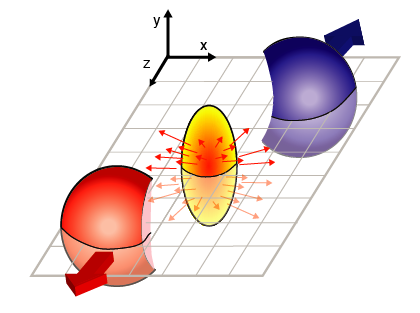
\includegraphics[width=0.38\linewidth]{images/illustration_1_initial_spatial_asymmetry.png}
  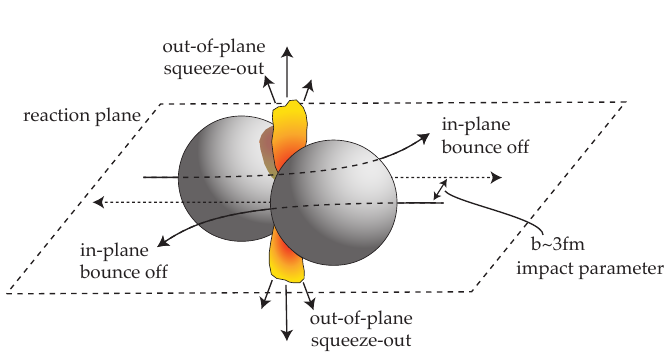
\includegraphics[width=0.55\linewidth]{images/flow1.png}
 \caption{ Cхематичное изображение механизмов происхождения направленного $v_1$ и эллиптического $v_2$ потоков в
  столкновениях ядер при энергиях $\sqrt{s_{NN}}>$ 25 ГэВ (слева) и $\sqrt{s_{NN}}$=2-4 ГэВ (справа).}
\label{fig:bounce_off}
\end{center}
\end{figure}

При высоких энергиях столкновения $\sqrt{s_{NN}} > 25$ ГэВ, когда время прохождения сталкивающихся ядер ($t_{pass}<$ 1 фм/c) меньше типичного времени расширение  материи в области перекрытия ядер ($t_{exp}$), в гармониках $v_n$ потока доминирует гидродинамическое коллективное расширение КГМ. 
Оно вызвано наличием начальной пространственной анизотропии области перекрытия ядер и геометрической флуктуации ее формы, которую можно охарактеризовать набором коэффициентов эксцентриситета $\varepsilon_n$, как схематически изображено на рис.~\ref{fig:bounce_off} (слева).
Константа пропорциональности между $v_n$  и $\varepsilon_n$ оказывается чувствительной к транспортным свойствам КГМ, таким как соотношения вязкости сдвига к плотности энтропии $\eta/s$.
Детальное сравнение модельных расчетов с измерениями $v_n$, что КГМ при энергиях RHIC и LHC по своим свойствам является сильновзаимодействующей, близкой к идеальной, жидкости со значением $\eta/s$, близким к постулированному минимуму 1/$(4\pi) \simeq$ 0.08.
Сравнение с расчетами транспортных моделей (RQMD, UrQMD и JAM), в которых нет формирования КГМ, показывают, что перерассеяние адронов может воспроизвести только 20-30\% от наблюдаемой величины сигнала  ($v_n$) потоков на RHIС.
В ходе программ сканирования по энергии на коллайдере RHIC от $\sqrt{s_{NN}}$ = 3.0 до 200 ГэВ коллаборацией STAR было получено много интересных результатов для коллективных потоков.
Наклон прямого потока $dv_1/dy$ в области средних быстрот ($y \sim 0$) для протонов и разницы между наклоном $dv_1/dy$ у протонов и анти-протонов показывает сильно немонотонную зависимость от энергии столкновения в области от 3.0 до 39 ГэВ. 
Это может указывать на “смягчение“ уравнения состояния в результате фазового перехода первого рода. 
Модельные расчеты показывают, что вклад взаимодействия рожденных частиц со спектаторами становится значительным для энергий столкновения менее чем $\sqrt{s_{NN}}\sim$7 ГэВ. 
Это приводит к росту сигнала направленного потока $v_1$ и уменьшению сигнала эллиптического потока $v_2$ нуклонов с уменьшением энергии столкновения. 
$v_2$ протонов меняет свой знак  от положительного к отрицательному при энергии около 4 ГэВ, см рис.~\ref{fig:bounce_off} (справа). 
В области энергий порядка $\sqrt{s_{NN}}\sim$ 2-5 ГэВ для описания $v_1$ и $v_2$ протонов необходимо использовать транспортные модели с импульсно-зависимым потенциалом среднего поля, такие как JAM~\cite{nara2019jam}.

Во втором разделе \underline{\textbf{первой главы}}  рассматриваются методы измерения азимутальных коллективных потоков, которые можно сформулировать в терминах  единичного вектора частиц $u_{n,k} = ( \cos n\varphi_k, \sin n\varphi_k )$ в плоскости поперечной оси пучка и
вектора потока $Q_n$ гармоники $n$:
\begin{equation}
    Q_n = \frac{1}{C} \sum_{k=1}^{N} w_k u_{n,k} = \frac{|Q_n|}{C} (\cos{\Psi_n}, \sin{\Psi_n}) ,
\end{equation}
где $\Psi_n$ --- угол плоскости симметрии данного события. 
Сумма проходит по всем частицам  в случае трекового детектора  или по модулям детекторов с азимутальной сегментацией. 
Угол $\varphi_k$ является азимутальным углом вылета частицы $k$ или азимутальной координатой $k$-го элемента сегментированного детектора. 
Для треков  вес $w_k$  может быть единицей или заданной функцией $p_T$. 
Для сегментированных детекторов в качестве веса $w_k$ используется сигнал, наблюдаемый в $k$-м сегменте детектора: заряд частиц или энергия. 
В методе плоскости события (EP) нормировочный коэффициент $C=|Q_n|$, а в методе  скалярного произведения (SP) нормировка производится на множественность частиц в $Q_n$:  $C=\sum_{k=1}^N w_k$. 
Тогда значение $v_n$ определяется как проекция $u_n$-вектора на плоскость симметрии события:
\begin{equation}
 % v_n = \frac{v_n^{obs}}{R_n} =  \frac{\langle u_n Q_n^* \rangle }{R_n}.\label{eq:v1_formula}
    v_n = v_n^{obs}/R_n =  \langle u_n Q_n^* \rangle/R_n, \label{eq:v1_formula}
\end{equation}
где $R_n$ - разрешение плоскости симметрии и угловые скобки обозначают среднее по всем частицам в событии и по всем событиям. 
Для вычисления $R_n$  используется метод, называемый методом трёх подсобытий:
%
\begin{equation}
    R_n\{a(b,c)\}  =  \sqrt { \frac{ \langle Q_n^a Q_n^b \rangle \langle Q_n^a Q_n^c \rangle }{ \langle Q_n^b Q_n^c \rangle} },
\end{equation}
%
где $a$, $b$ и $c$ --- три различных группы частиц, в каждой из которых $Q_n$-вектор вычислялся независимо.
Сравнивая $v_n$ полученный относительно различных плоскостей симметрии (к примеру, $v_n\{a\}$ и $v_n\{b\}$), можно оценить вклад непотоковых корреляций в результаты измерения. 

Неоднородность азимутального аксептанса детектора  искажает распределение $Q_n$-вектора, которое в идеальном случае должно быть равномерным. 
Для коррекции этого эффекта был использован метод, описаный в работе~\cite{Selyuzhenkov:2007zi}.
Поскольку плоскость реакции распределена равномерно, формулу~(\ref{eq:v1_formula}) можно преобразовать следующим образом:
%
\begin{equation}
  %  v_n =  2\frac{ \langle x_n X_n \rangle }{R_n^X} = 2\frac{ \langle y_n Y_n \rangle }{R_n^Y},
    v_n =  2 \langle x_n X_n \rangle/R_n^X = 2 \langle y_n Y_n \rangle/R_n^Y,
    \label{eq:v1xy_formula}
\end{equation}
%
где $x_n$ и $y_n$ --- компоненты $u_n$-вектора, $X_n$ и $Y_n$ --- компоненты $Q_n$-вектора и $R_n^{X,Y}$ --- разрешение плоскости симметрии, вычисленное при помощи корреляций компонент $Q_n$-векторов.
Систематический вклад азимутальной неоднородности аксептанса детектора может быть оценен сравнением результатов полученных с использованием различных компонент $u_n$ и $Q_n$-векторов. 
В области энергий 1-4 АГэВ направленный поток $v_1$ является доминирующем сигналом, который не меняет свой знак,  поэтому $v_1$ и более высокие гармоники вычисляются относительно  плоскости симметрии первой гармоники $\Psi_1$.\\

\underline{В первом разделе \textbf{второй главы}} приведено описание эксперимента на фиксированной мишени  HADES~\cite{HADES:2009aat}, который 
состоит из тороидального сверхпроводящего магнита, центрированного вокруг оси пучка, с шестью одинаковыми секторами регистрации, см. рис.~\ref{fig:hades_bmn_layouts} (слева).
Трекинговая система, состоит из четырёх плоскостей многопроволочных дрейфовых камер (MDC).
Идентификация заряженных частиц проводится одновременно  используя  времяпролётную систему TOF$+$RPC и по энерговыделению в камерах MDC.
Сцинтилляционный годоскоп Forward Wall (FW), расположенный на расстоянии 6.8 m от мишени, предназначен для регисмтрации заряженных фрагментов спектаторов налетающего ядра.
%
\begin{figure}[h]
\begin{center}
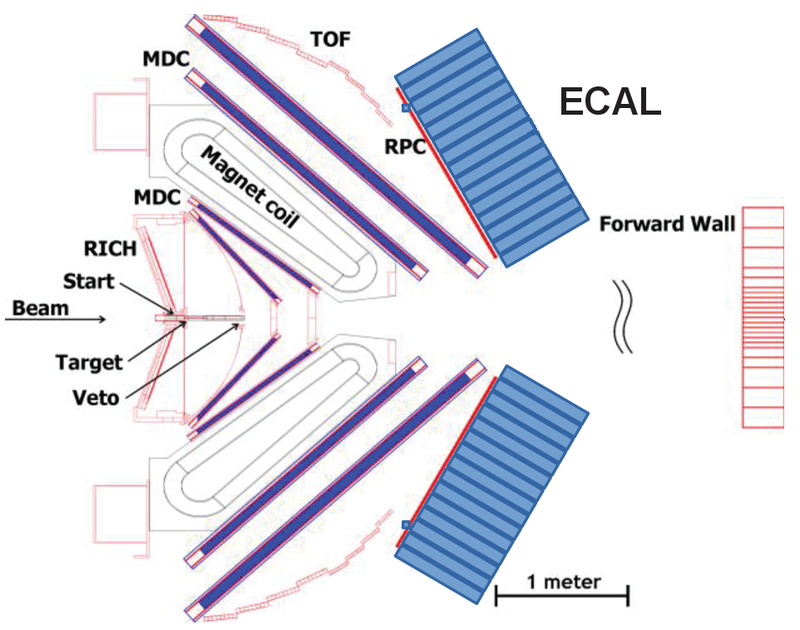
\includegraphics[width=0.37\linewidth]{images/hades_layout.jpg}
%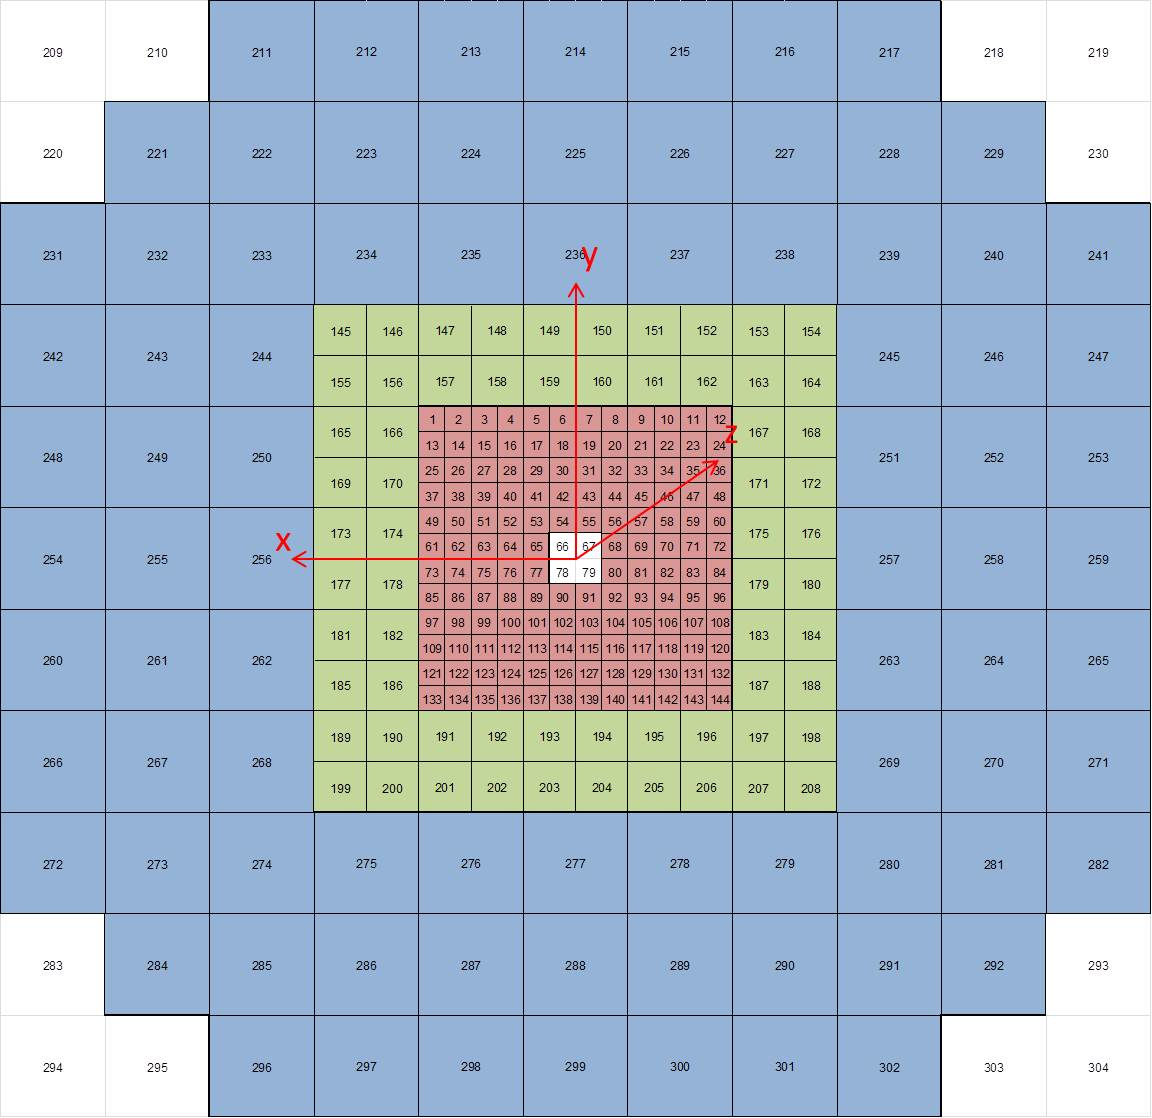
\includegraphics[width=0.35\linewidth]{images/FW_layout.jpg}
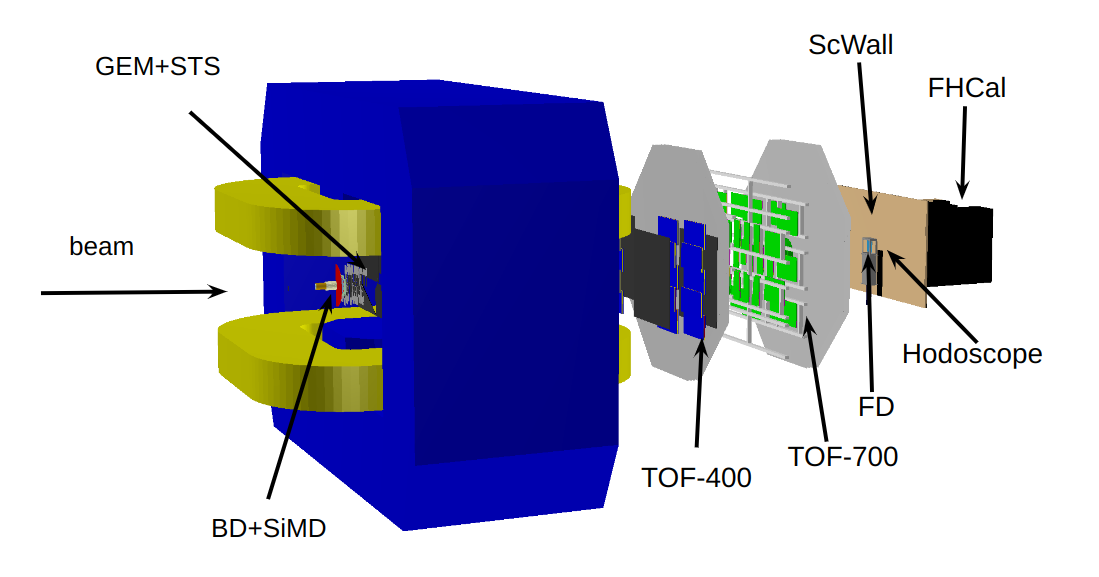
\includegraphics[width=0.55\linewidth]{images/BM@N_layout.png}
\caption{Схема экспериментов HADES (слева) и BM@N (справа).}
\label{fig:hades_bmn_layouts}
\end{center}
\end{figure}

\underline{Во втором разделе \textbf{второй главы}} представлено краткое описание экспериментальной установки BM@N (см. рис.~\ref{fig:hades_bmn_layouts} (справа)).
Центральная трековая система BM@N состоящая из 4 станций двусторонних кремниевых микрополосковых датчиков (STS) и 7 станций камер газообразных электронных умножителей (GEM) расположена внутри дипольного магнита с большой апертурой, что позволяет восстанавливать импульс $p$ заряженных частиц c разрешением  $\Delta p/p \sim$ 1.7-2.5$\%$ для энергий порядка 3.5--4A~ГэВ. 
Время-пролетная система, состоящая из двух детекторов TOF400 и TOF700, используется для идентификации заряженных частиц.
Три передних детектора: передний адронный калориметр (FHCal), кварцевый годоскоп (Hodo) и  сцинтилляционная стенка (ScWall) предоставляют информацию о фрагментах спектаторов налетающего ядра.
В феврале 2023 года закончился первый  набор физических данных, в ходе которого BM@N набрал порядка 500 М событий столкновений ядер Xe+Cs(I) при энергии  $E_{kin}$ = 3.8 АГэВ.

\underline{\textbf{Третья глава}} Расматривается разработанная автором методика измерения направленного потока $v_1$ протонов в эксперименте HADES~\cite{Mamaev:2020lpi,HADES:2020lob,Mamaev:2020qom}. 
Первая часть посвящена отбору событий для анализа. 
Для анализа использовались только события столкновений, вершина которых лежала в следующих границах: $\sqrt{x_v^2+y_v^2}<3$~мм и $z_v \in (-60, 0)$~мм.
Треки частиц были выбраны в соответствии с параметром качества $\chi^2<100$, предоставленным алгоритмом фитирования трека, и ограничением на минимальное расстояние сближения трека с вершиной (DCA): $(-10,10)$~mm. 
Протоны идентифицировались при помощи информации из системы  TOF+RPC (см. рис.~\ref{fig:hades_pid} (слева)).

\begin{figure}[h]
\begin{center}
  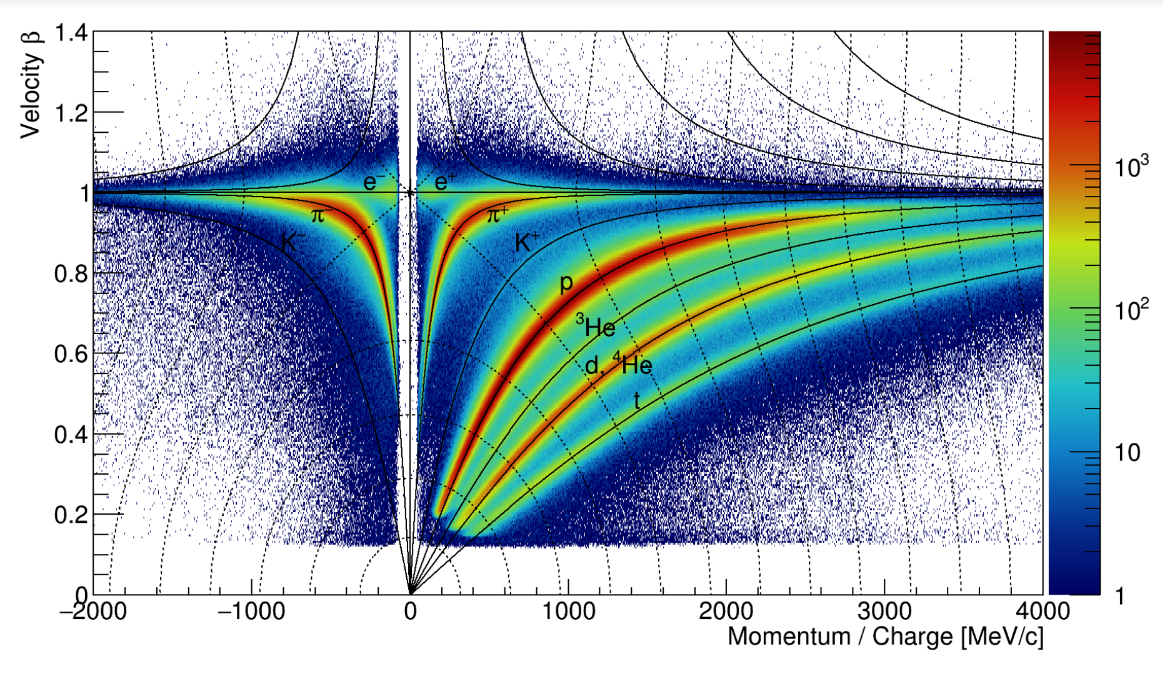
\includegraphics[width=0.54\linewidth]{images/hades_pid_plot.png}
  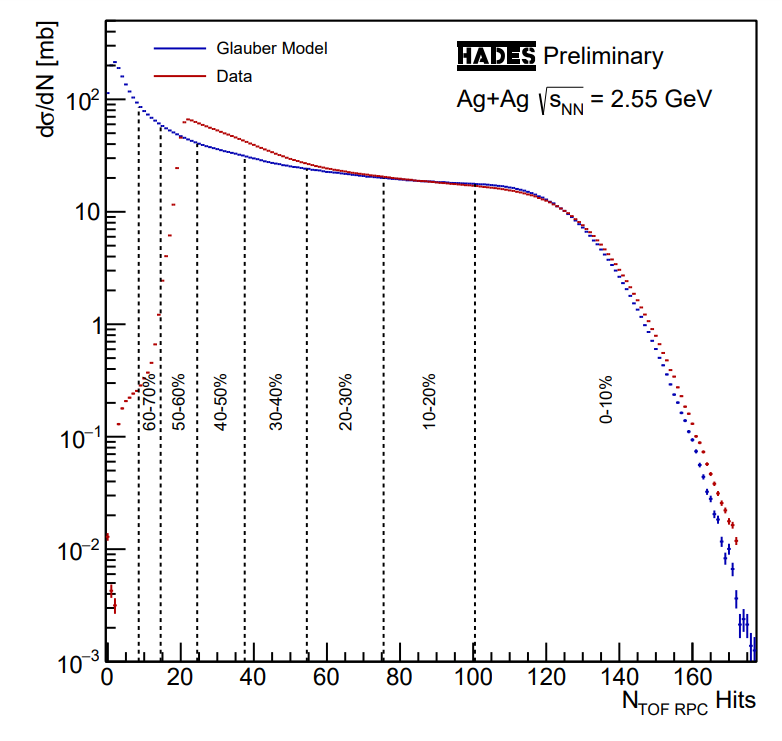
\includegraphics[width=0.33\linewidth]{images/hades_mult.png}
  \caption{ Слева: распределение частиц со скоростью $\beta$  в зависимости от  импульса частицы к заряду
    (p/q). Справа: пример распределения суммарной множественности хитов в системе TOF+RPC.}
\label{fig:hades_pid}
\end{center}
\end{figure}

Распределение суммарной множественности хитов в системе TOF+RPC было использовано для определения центральности столкновений, используя метод подгонки Монте-Карло версией модели Глаубера ~\cite{HADES:2017def}(см. рис.~\ref{fig:hades_pid} (справа)).

\begin{figure}[h]
\begin{center}
  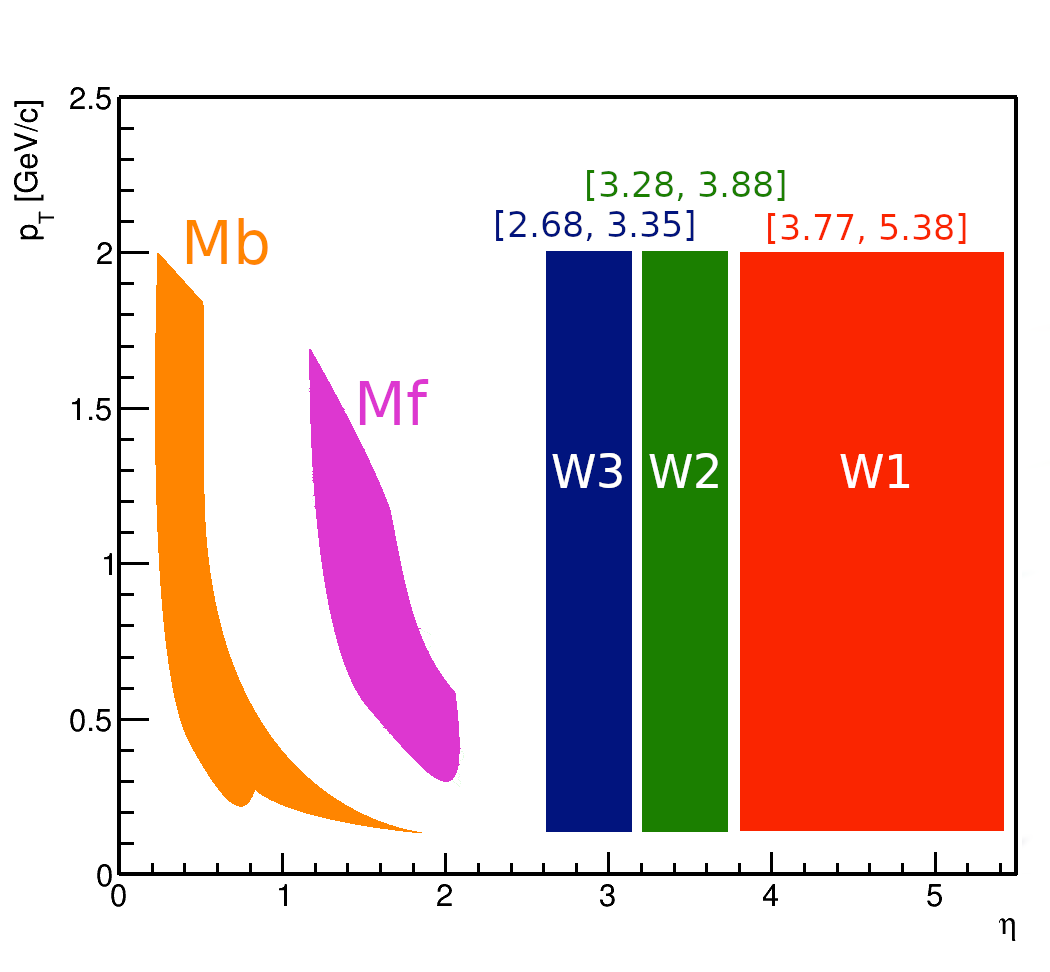
\includegraphics[width=0.37\linewidth]{images/eta_pt_qvectors.png}
   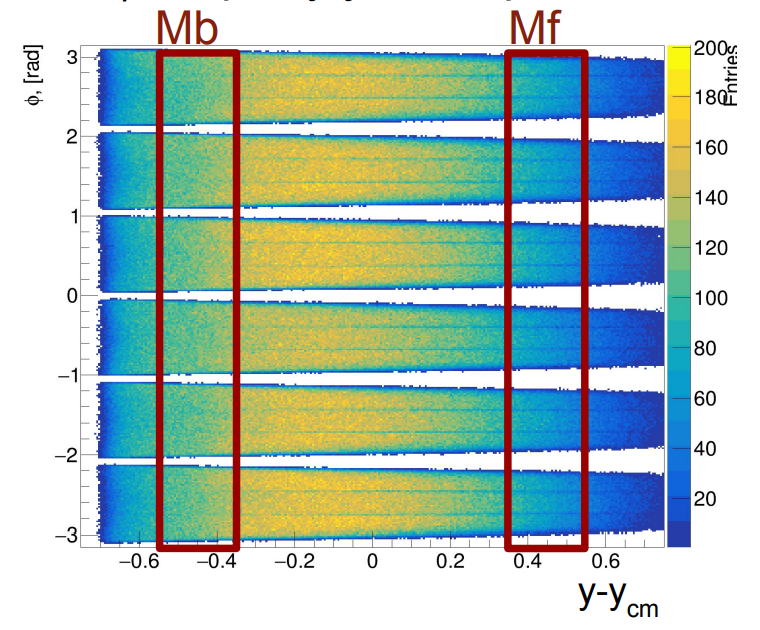
\includegraphics[width=0.39\linewidth]{images/hades_phi_rapidity.png}
   \caption{ Схематическое изображение аксептанса $p_T$ vs $\eta$, использованного для построения пяти  $Q_1$ -векторов для анализа $v_1$ протонов (слева).
   Азимутальный аксептанс  протонов в плоскости $\phi$  vs $y_{cm}$ (справа). }
\label{fig:hades_qvectors}
\end{center}
\end{figure}
%
Для оценки плоскости симметрии модули детектора FW были разделены на 3 группы: центральные (W1), средние (W2) и периферические (W3). 
Это позволило определить три $Q_1$ -вектора, см. рис.~\ref{fig:hades_qvectors} (слева).
Для оценки систематической ошибки вызванной непотоковыми корреляциями были построены 2 дополнительных $Q_1$-вектора из треков протонов, см. рис~\ref{fig:hades_qvectors} (справа).
Рисунок~\ref{fig:hades_uq_corr} показывает сравнение $v_1^{uncor}$ протонов, полученного с использованием различных компонент $u_1$ и $Q_1$-векторов~\cite{Mamaev:2020qom}. 
После применения поправок на азимутальную анизотропию аксептанса, остаточный эффект составляет порядка 2\%.\\
%
\begin{figure}[h]
\begin{center}
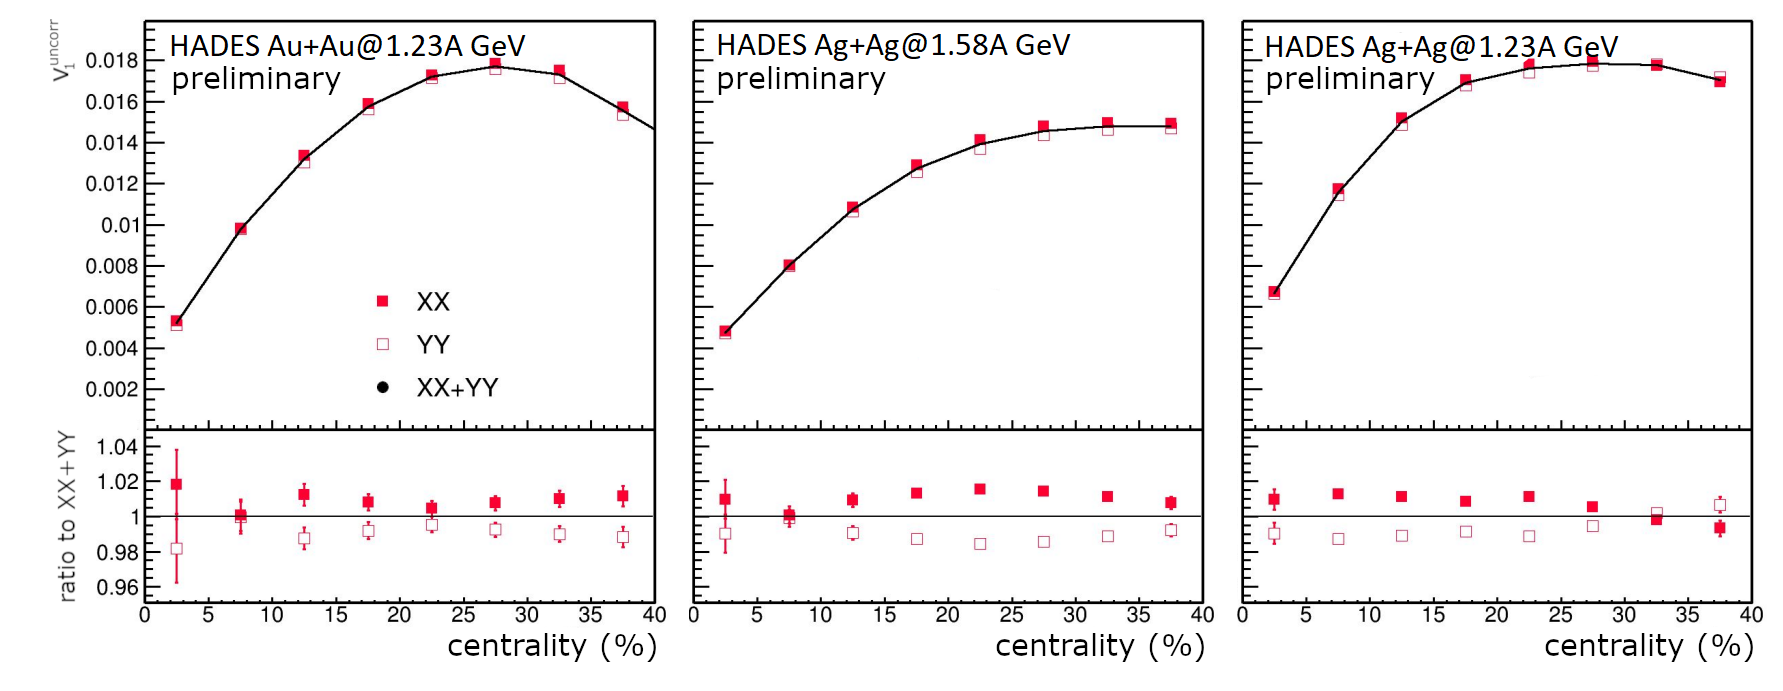
\includegraphics[width=0.75\linewidth]{images/hades_u1W1_centrality.png}
\caption{Зависимость компонент корреляции $\langle u_1 Q_1 \rangle$ от центральности после применения поправок на азимутальную неоднородность детектора.}
 %для  Au+Au и Ag+Ag столкновений.}
\label{fig:hades_uq_corr}
\end{center}
\end{figure}

Разрешение плоскости симметрии $R_1$, полученное с использованием различных комбинаций $Q_1$-векторов, показано на рис~\ref{fig:hades_w1_combinations}~\cite{Mamaev:2020qom}.
Разрешение $R_1\{W1(W2,W3)\}$ заметно отличается от значений, полученных при помощи других комбинаций. 
Этот эффект может быть объяснён наличием непотоковых корреляций между парами $Q_1$-векторов $W1$ и $W2$, $W2$ и $W3$, которые не имеют значительного разделения по быстроте. 
В столкновениях Ag+Ag при обеих энергиях, $R_1\{W1(Mf,Mb)\}$ так же значительно отклоняется от среднего результата. 
Это может быть вызвано наличием корреляций из-за закона сохранения импульса между векторами $Mf$ и $Mb$. 
Для Au+Au этот эффект менее выражен в силу большей множественности рождённых частиц.

\begin{figure}[h]
\begin{center}
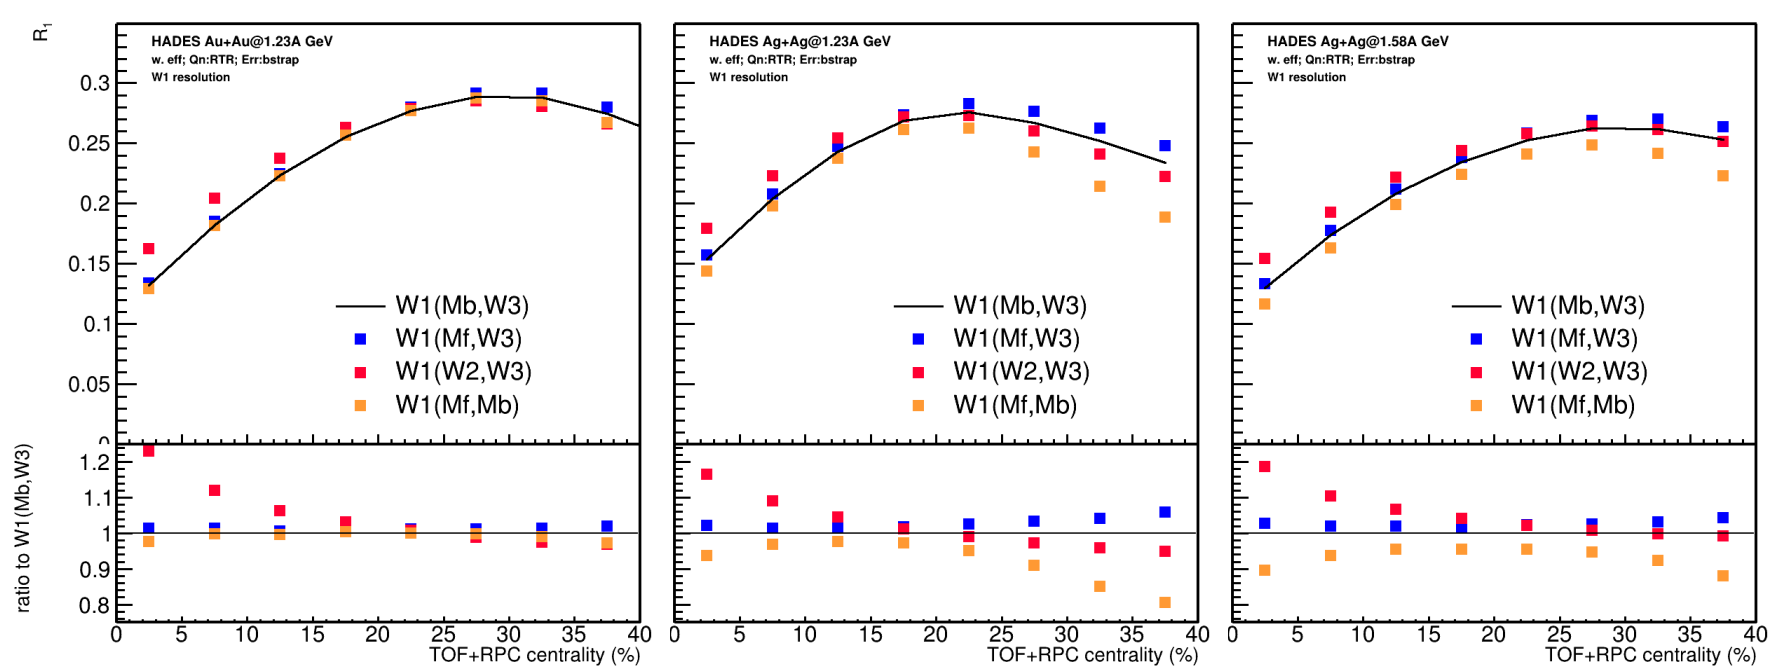
\includegraphics[width=0.75\linewidth]{images/W1_combinations.png}
\caption{Зависимость  разрешения $R_1$ от центральности для различных комбинаций $Q_1$-векторов
  для Au+Au и  Ag+Ag столкновений}
\label{fig:hades_w1_combinations}
\end{center}
\end{figure}

\begin{figure}[h]
\begin{center}
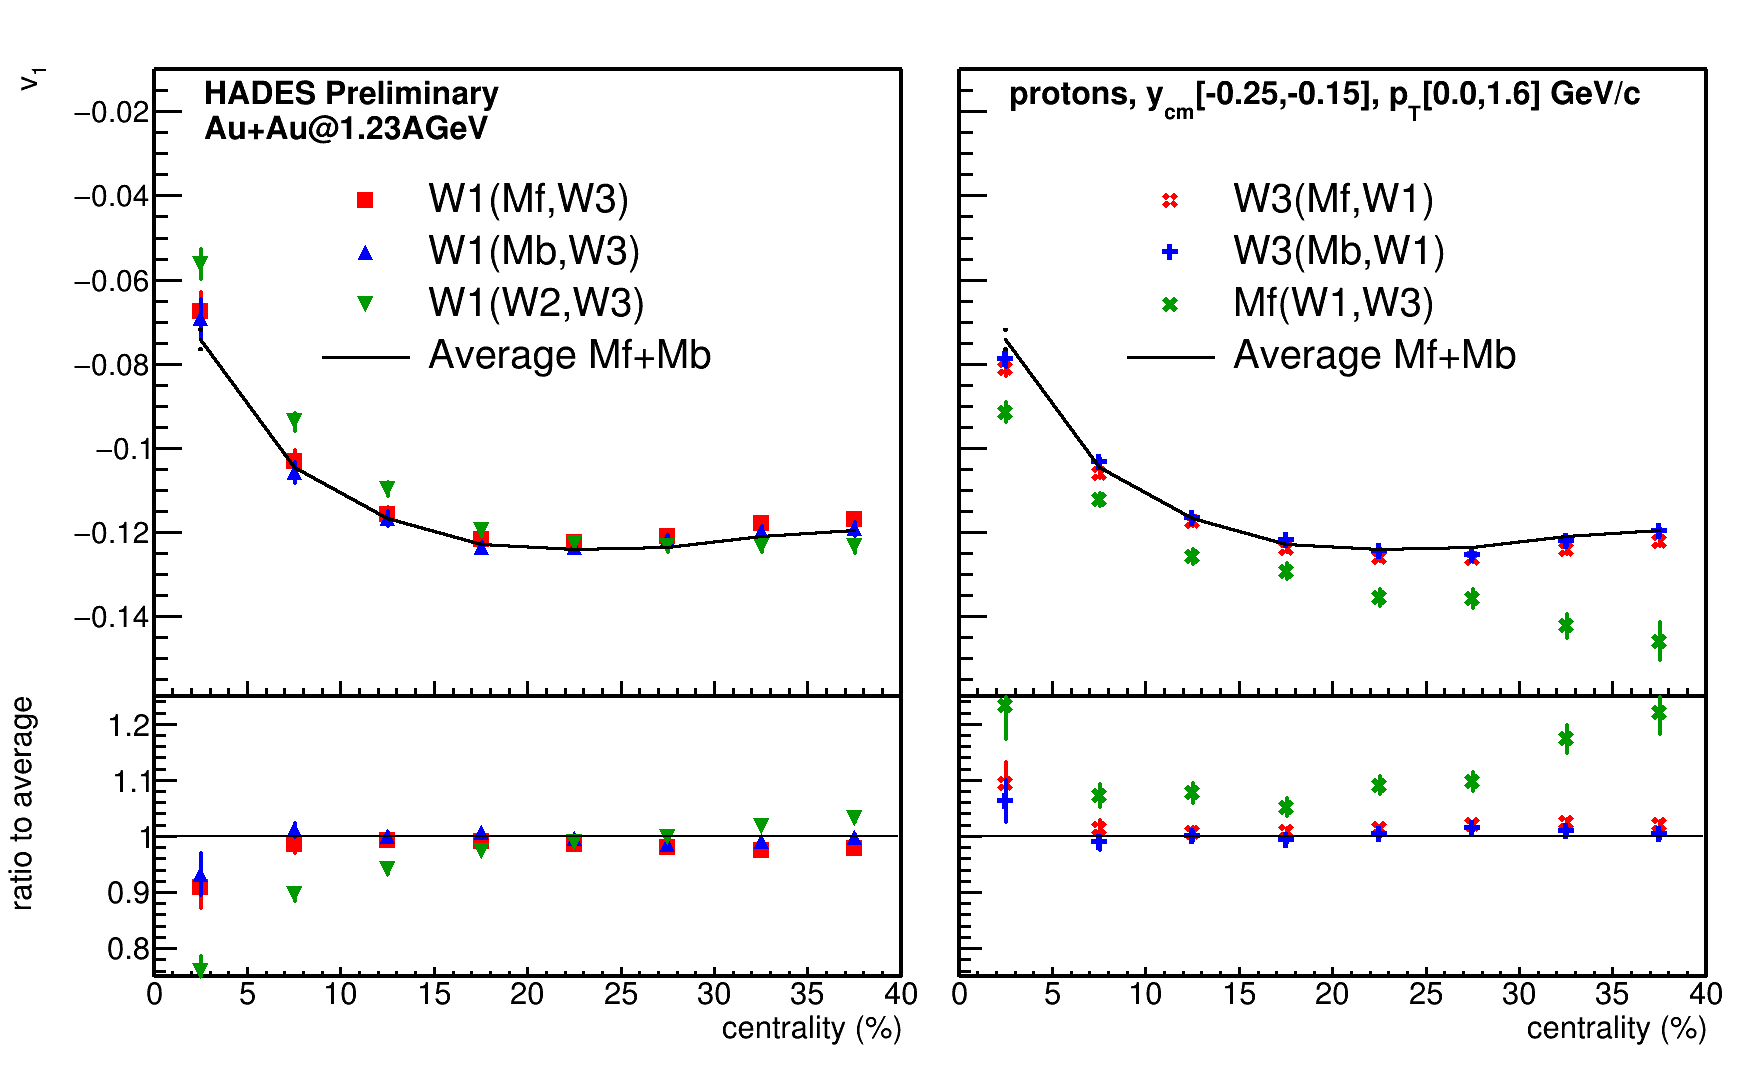
\includegraphics[width=0.65\linewidth]{images/W1AndW3Nucleus.png}
\caption{Зависимость $v_1$ протонов от центральности  в столкновениях Au+Au,
  измеренная при помощи различных комбинаций $Q_1$-векторов. }
\label{fig:hades_w1w3}
\end{center}
\end{figure}
На рис.~\ref{fig:hades_w1w3} представлена зависимость  $v_1$ протонов от центральности  в столкновениях Au+Au при $E_{kin}=$1.23$A$~ГэВ, измеренная при помощи различных комбинаций $Q_1$-векторов~\cite{Mamaev:2020qom}.
Слева представлены значения $v_1$ измеренные относительно внутреннего подсобытия W1, справа --- внешнего подсобытия W3 и подсобытия из треков заряженных частиц Mf. 
Результаты для комбинаций подсобытий, разделенных по быстроте, таких как например, $W1(Mf,W3)$ и $W1(Mb,W3)$ согласуются между собой в пределах 2\%, за исключением наиболее центральных событий. 
Значения $v_1$, измеренные относительно различных плоскостей симметрии $W1$ и $W3$, так же согласуется в пределах 2\%.
Результаты для $v_1$, полученные с использованием комбинаций не разделенных по быстроте $Q_1$-векторов (например $W1(W2,W3)$) значительно отличаются.
В дальнейшем в качестве значений $v_1$ протонов было использовано среднее по всем комбинациям $Q_1$-векторов, разделенных по быстроте.

В  \underline{\textbf{четвертой главе}} приведены основные результаты измерения направленного потока $v_1$ протонов в  эксперименте HADES и результаты исследования эффективности измерениия $v_n$ протонов в
эксперименте BM@N.

На рис.~\ref{fig:hades_prl} показана зависимость измеренного направленного потока  $v_1$ протонов от поперечного импульса $p_T$ (слева) и быстроты $y_{cm}$ для 20-30\% центральных Au+Au столкновений при кинетической энергии пучка $E_{kin}=1.23A$~ГэВ ~\cite{HADES:2020lob}. 
Для сравнения также показаны значения $v_1$   для дейтронов и тритонов.

\begin{figure}[h]
\begin{center}
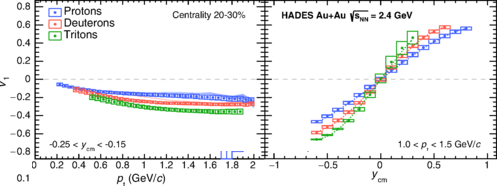
\includegraphics[width=0.75\linewidth]{images/HADES_prl.png}
\caption{$v_1$($p_T$) (слева) и  $v_1$($y_{cm}$) (справа)  для протонов, дейтронов и тритонов  в  Au+Au столкновениях при
  энергии $E_{kin}=$1.23$A$~ГэВ.}
\label{fig:hades_prl}
\end{center}
\end{figure}

На рисунке~\ref{fig:hades_v1_ycm_pT} представлена зависимость  $v_1$ протонов от быстроты  $y_{cm}$  (слева) и поперечного импульса $p_T$ (справа) для среднецентральных Au+Au  и  Ag+Ag  столкновений~\cite{Mamaev:2024-1, Mamaev:2024-2}. 
Типичными источниками погрешностей измерений $v_1$ и их характерными относительными значениями являются: 
погрешности в реконструкции треков и определении импульса частиц (1-3\%) в зависимости от $p_T$ и $y_{cm}$; 
из­менения критериев отбора кандидатов в протоны по квадрату массы (1-3\%); 
остаточная  разница между компонентами $XX$ и $YY$ корреляции векторов $u_1$ и $Q_1$ (1-2\%);
сравнение результов полученных методами плоскости события и скалярного произведения (1-4\%); 
вклад непотоковых корреляций, путем сравнения значений $v_1$, полученных относительно различных плоскостей симметрии (W1, W2, W3) и деленных на поправочный коэффициент разрешения, рассчитанный с использованием различных комбинаций $Q_1$-векторов (3-5\%)~\cite{Mamaev:2020lpi, HADES:2020lob,Mamaev:2020qom}.

Значения $v_1$ протонов, в столкновениях Au+Au и Ag+Ag при  энергии $E_{kin}=$1.23$A$~ГэВ, хорошо согласуются с учетом систематических ошибок. 
Протоны, рожденные в столкновениях Ag+Ag при большей энергии $E_{kin}=$1.58$A$~ГэВ обладают меньшим значением $v_1$.
Модель JAM~\cite{nara2019jam} с импульсно зависимым потенциалом среднего поля хорошо описывает зависимость $v_1$ от быстроты $y_{cm}$, как показано линиями на рис~\ref{fig:hades_v1_ycm_pT}. 
Однако модель не способна описать зависимость $v_1$ протонов от поперечного импульса $p_T$.
%
\begin{figure}[h]
\begin{center}
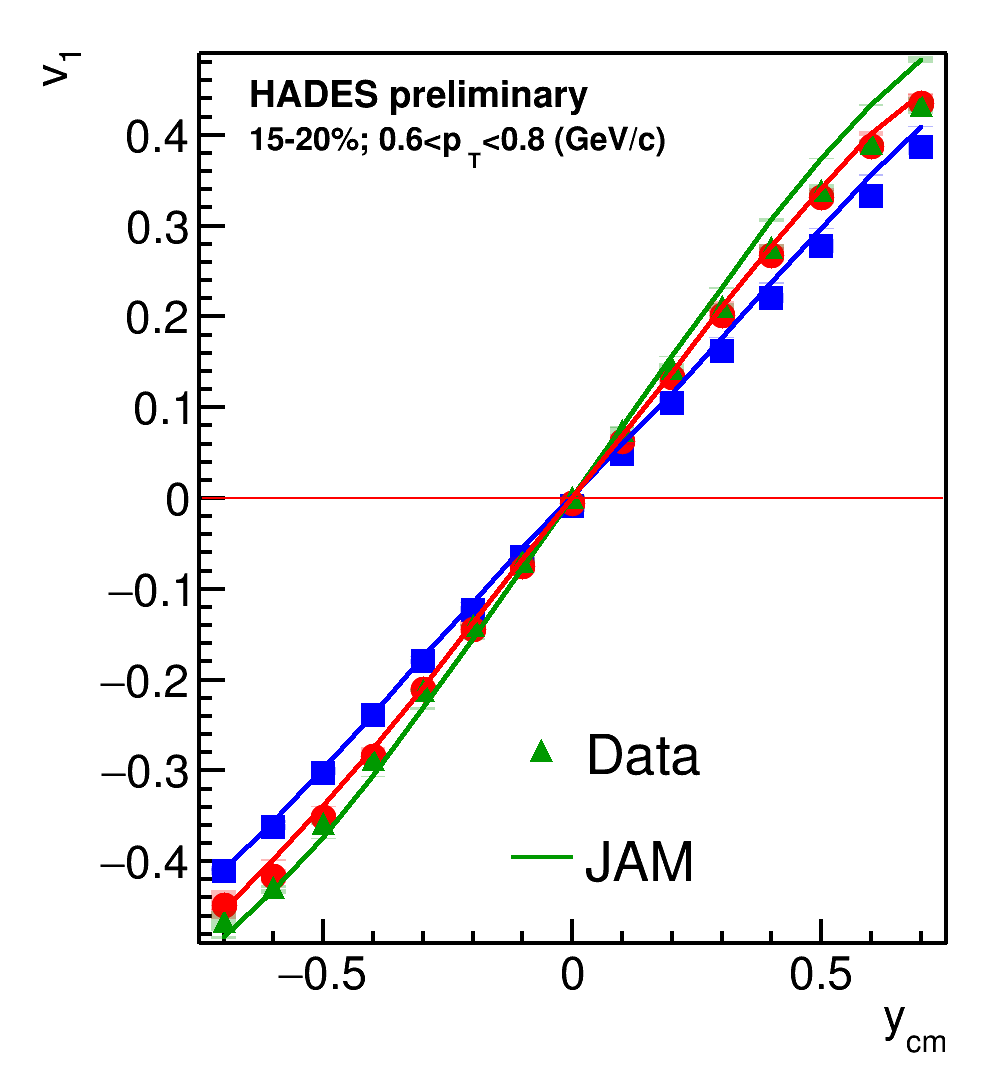
\includegraphics[width=0.38\linewidth]{images/v1_hades_ycm.png}
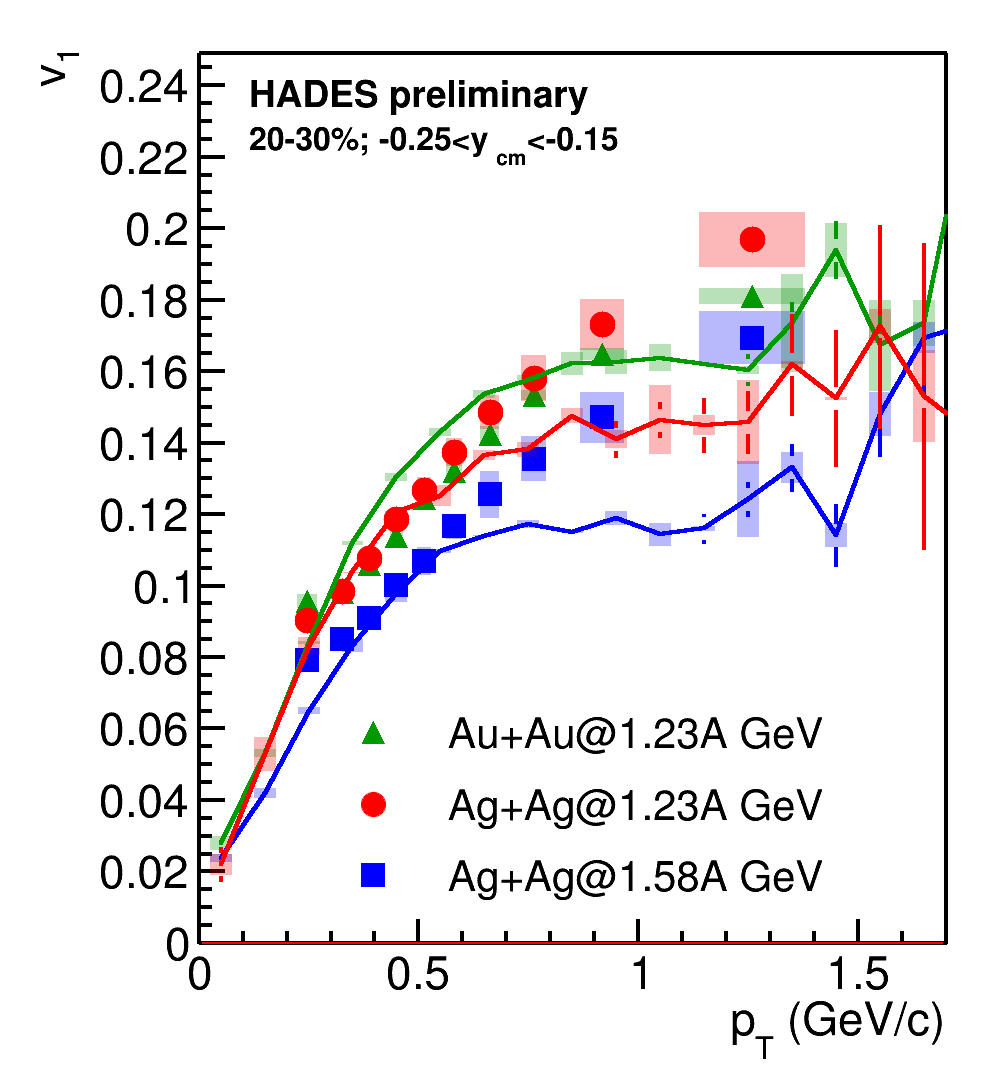
\includegraphics[width=0.38\linewidth]{images/v1_hades_pT.png}
\caption{Зависимость $v_1$ от  $y_{cm}$ (слева)  и $p_T$ (справа) для столкновений Au+Au и Ag+Ag. Линиями показаны данные, полученные из модели JAM.}
\label{fig:hades_v1_ycm_pT}
\end{center}
\end{figure}

Зависимость  $v_1$ протонов от  быстроты $y_{cm}$ была параметризована кубической функцией $v_1(y_{cm}) = a_0 + a_1 y_{cm} + a_3 y_{cm}^3$. 
Затем, наклон направленного потока  $dv_1/dy_{cm}|_{y_{cm}=0}$ в области средних быстрот $y_{cm}\sim0$ был извлечен как параметр $a_1$.
Полученные значения $dv_1/dy|_{y_{cm}=0}$ протонов в столкновениях \au{}  и \ag{} хорошо согласуются с измерениями  других экспериментов ~\cite{FOPI:2011aa,STAR:2020dav} (см. рис. ~\ref{fig:hades_dv1_dy_sqrt_snn})~\cite{Mamaev:2024-1,Mamaev:2024-2}.
%
\begin{figure}[h]
\begin{center}
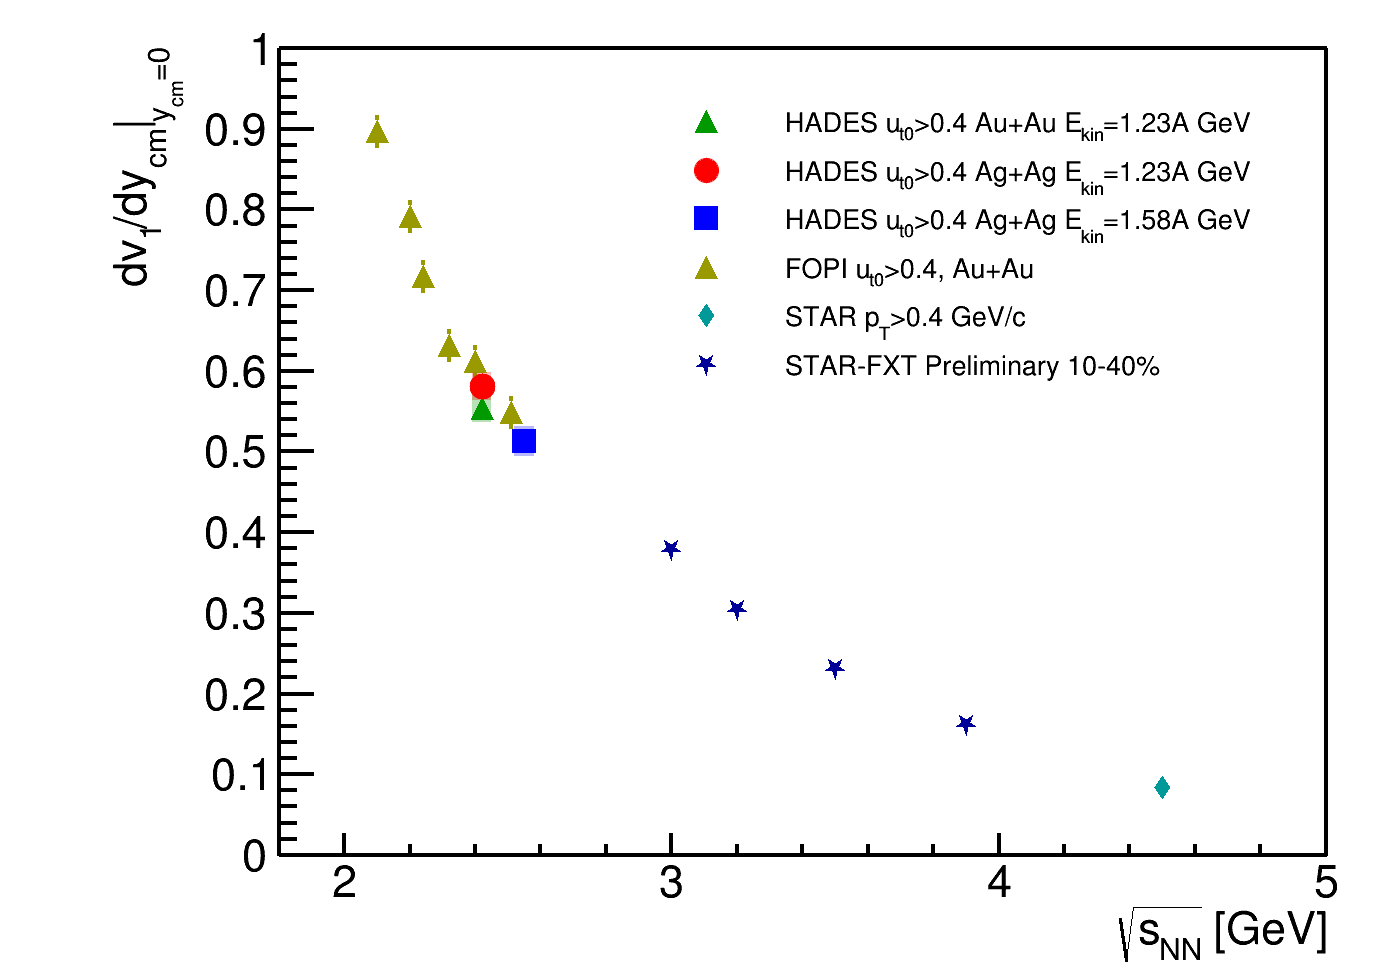
\includegraphics[width=0.47\linewidth]{images/dv1_dy_sqrt_snn.png}
\caption{ 
  Зависимость $dv_1/dy|_{y_{cm}=0}$ протонов в среднецентральных столкновениях от  энергии столкновения $\sqrt{s_{NN}}$.
}
\label{fig:hades_dv1_dy_sqrt_snn}
\end{center}
\end{figure}


На рис.~\ref{fig:hades_dv1dy_many_plot} слева приведена зависимость наклона $dv_1/dy_{cm}|_{y_{cm}=0}$ протонов от центральности столкновения.
Поскольку при большей энергии время пролета двух ионов $t_{pass}$ меньше, наклон направленного потока протонов в столкновениях Ag+Ag при энергии $E_{kin}=$1.58$A$~ГэВ заметно меньше, чем при $E_{kin}=$1.23$A$~ГэВ. 
Для коррекции на время $t_{pass}$, наклон  $dv_1/dy_{cm}|_{y_{cm}=0}$ был нормирован на быстроту пучка $y_{beam}$: $dv_1/dy'|_{y'=0}$, где $y'=y_{cm}/y_{beam}$.
За исключением наиболее центральных событий, зависимость наклона $dv_1/dy'|_{y'=0}$ от центральности описывается одной кривой для всех трех наборов данных, см. центральную часть рис.~\ref{fig:hades_dv1dy_many_plot}.
В каждом классе центральности был вычислен средний прицельный параметр $\langle b \rangle$ из модели Глаубера.
Радиус ядра пропорционален корню кубическому из массового числа $r_N \propto A^{1/3}$.
Для учета зависимости от размера сталкиваемых ядер,  $\langle b \rangle$ в каждом классе по центральности был нормирован на $A^{1/3}$.
Наклон $dv_1/dy'|_{y'=0}$ как функция относительного прицельного параметра $\langle b \rangle / A^{1/3}$ представлен на рис~\ref{fig:hades_dv1dy_many_plot} справа.
Данное преобразование улучшило согласие зависимостей наклона в центральных событиях~\cite{Mamaev:2024-1,Mamaev:2024-2}. 
%
\begin{figure}[h]
\begin{center}
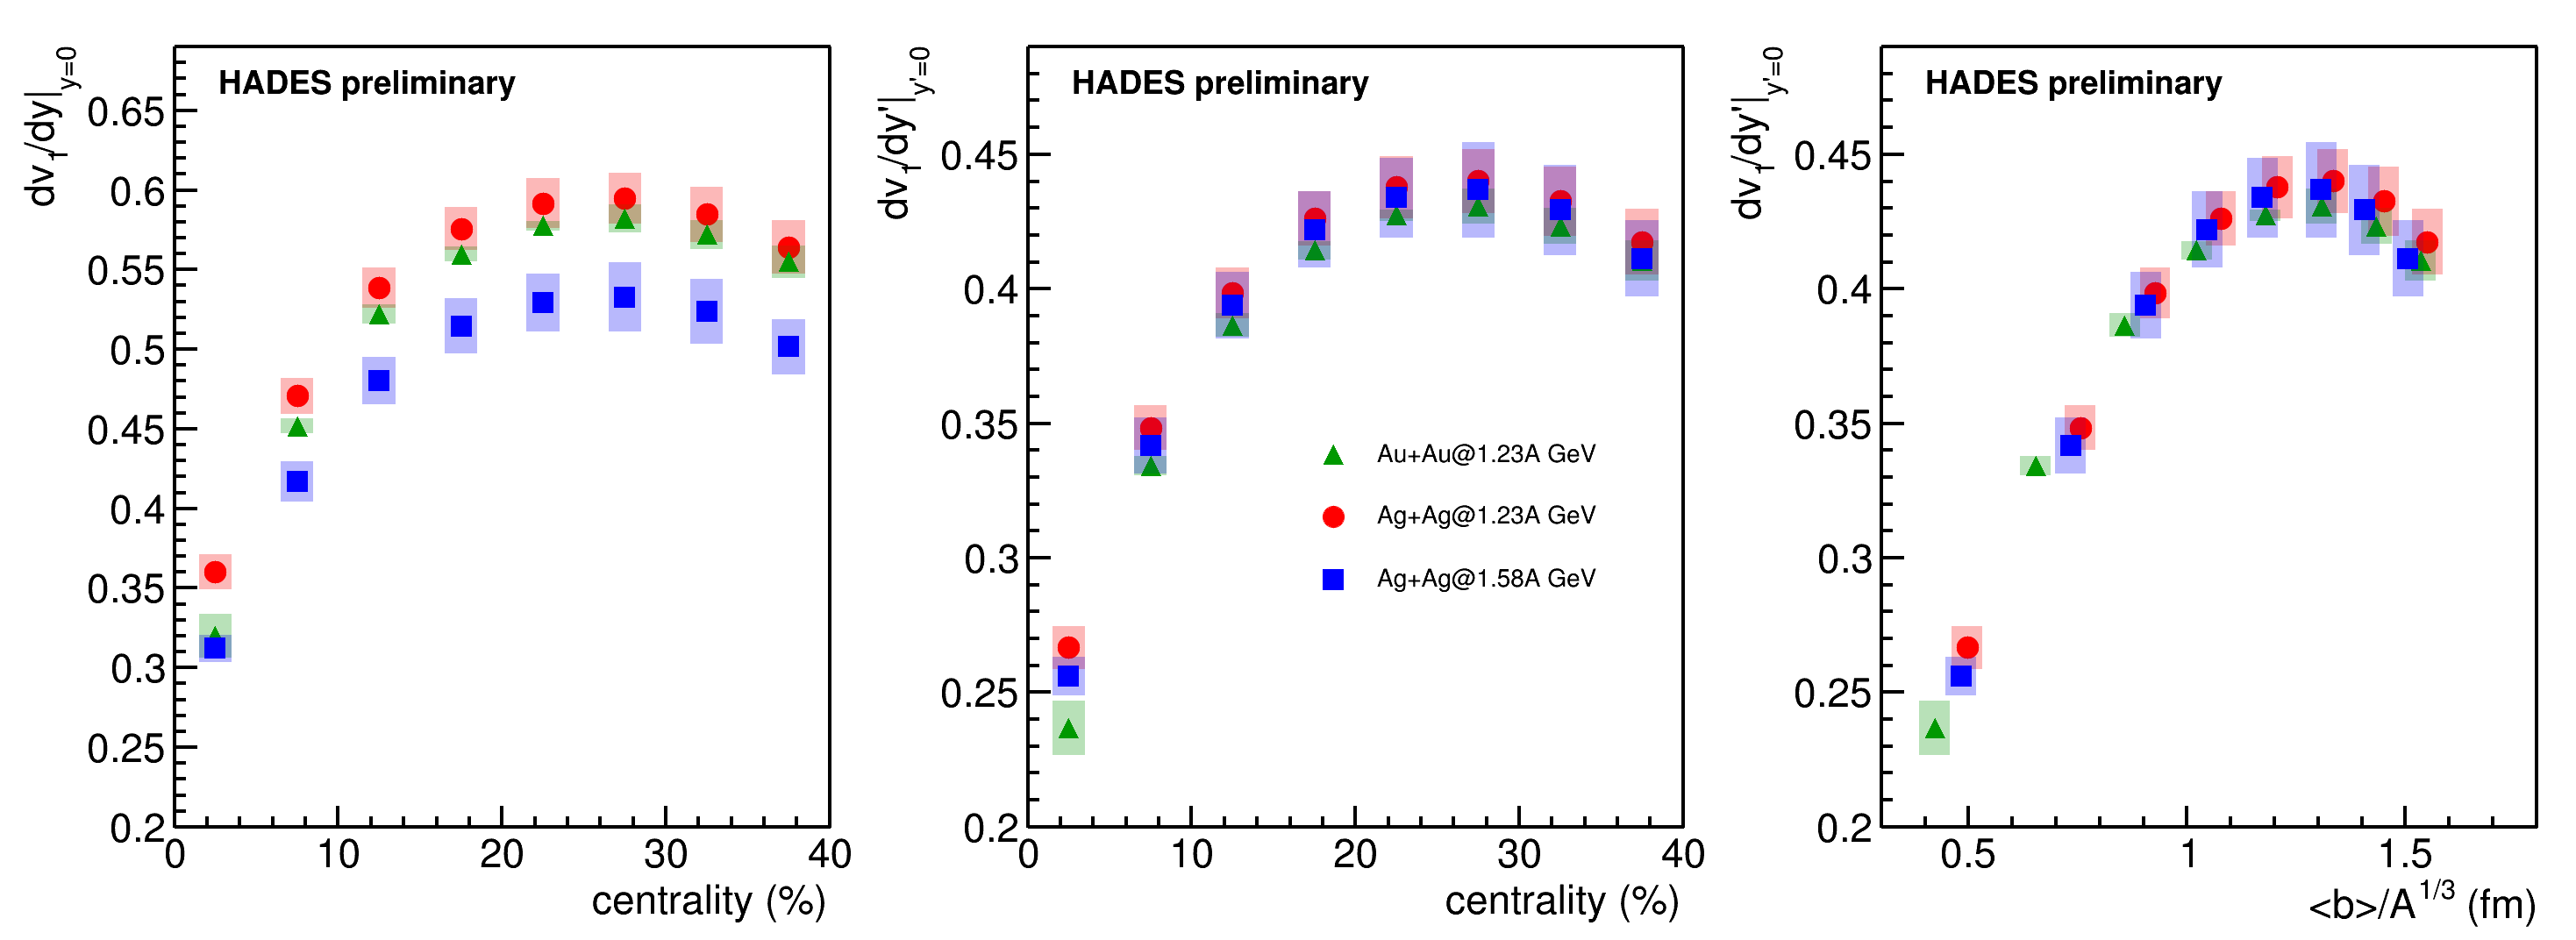
\includegraphics[width=0.9\linewidth]{images/dv1dy_many_plot.png}
\caption{Зависимость $dv_1/dy|_{y=0}$ протонов от центральности: (слева) для $y=y_{cm}$, (в центре) для $y_{cm}$ номированной 
на быстроту пучка $y' = y_{cm}/y_{beam}$ и (справа) для $dv_1/dy'|_{y'=0}$ как функции $\langle b \rangle$ нормированного на  $A^{1/3}$.}
\label{fig:hades_dv1dy_many_plot}
\end{center}
\end{figure}


Во второй части \underline{\textbf{четвертой главы}} приведены результаты изучения возможности измерения $v_1$ и $v_2$ протонов в столкновениях Xe+Cs(I)   в эксперименте  BM@N~\cite{Mamaev:2024,Mamaev:2023yhz,Mamaev:2023fpr}.
Эффективность  измерений была проверена  с помощью Монте-Карло моделирования   и последующий полной реконструкции событий в среде BMNROOT. 
Для восстановления плоскости симметрии модули адронного калориметра FHCal были разделены на 3 группы согласно их псевдобыстроте (F1, F2 и F3), см. рис.~\ref{fig:bmn_subevents} слева. 
Для исследования вклада непотоковых корреляций в результаты измерений были введены два дополнительных  $Q_1$-вектора из треков протонов $Tp$ и отрицательных пионов $T\pi$, см.  рис.~\ref{fig:bmn_subevents} справа.

\begin{figure}[h]
\begin{center}
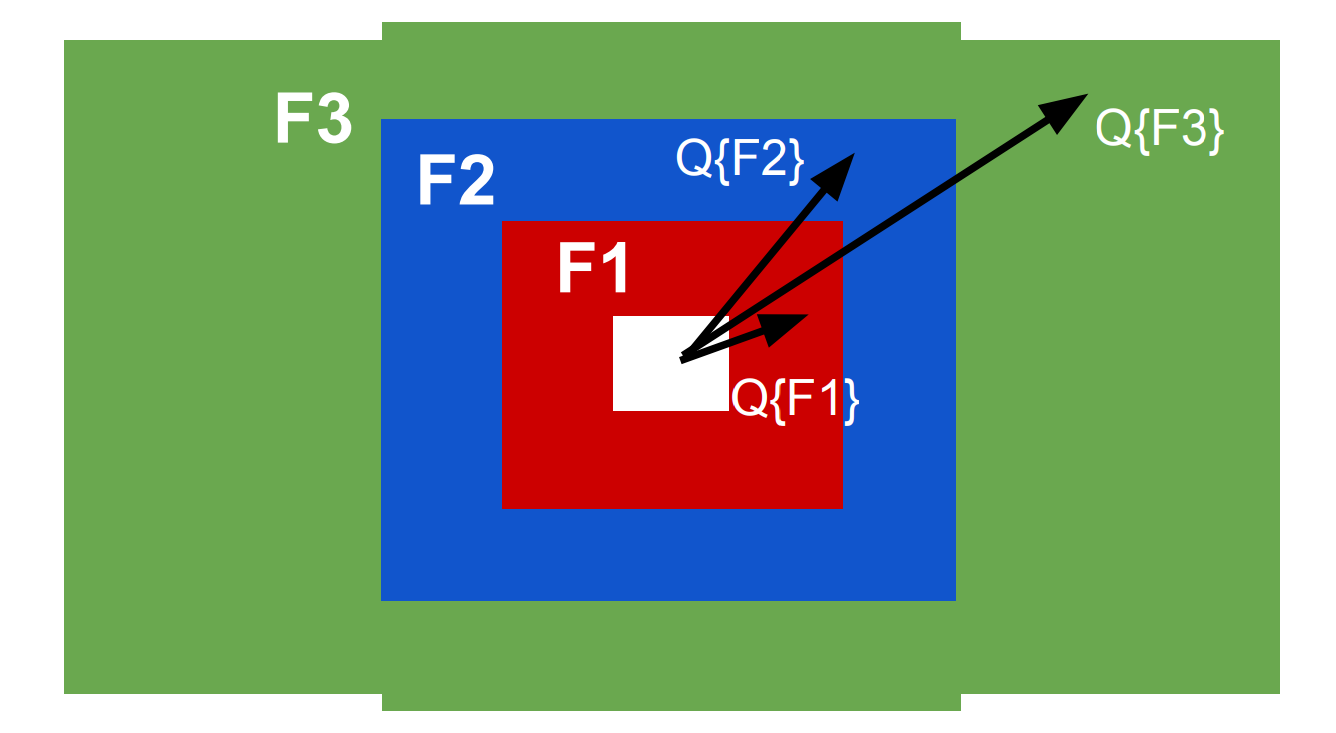
\includegraphics[width=0.45\linewidth]{images/FHCal_layout.png}
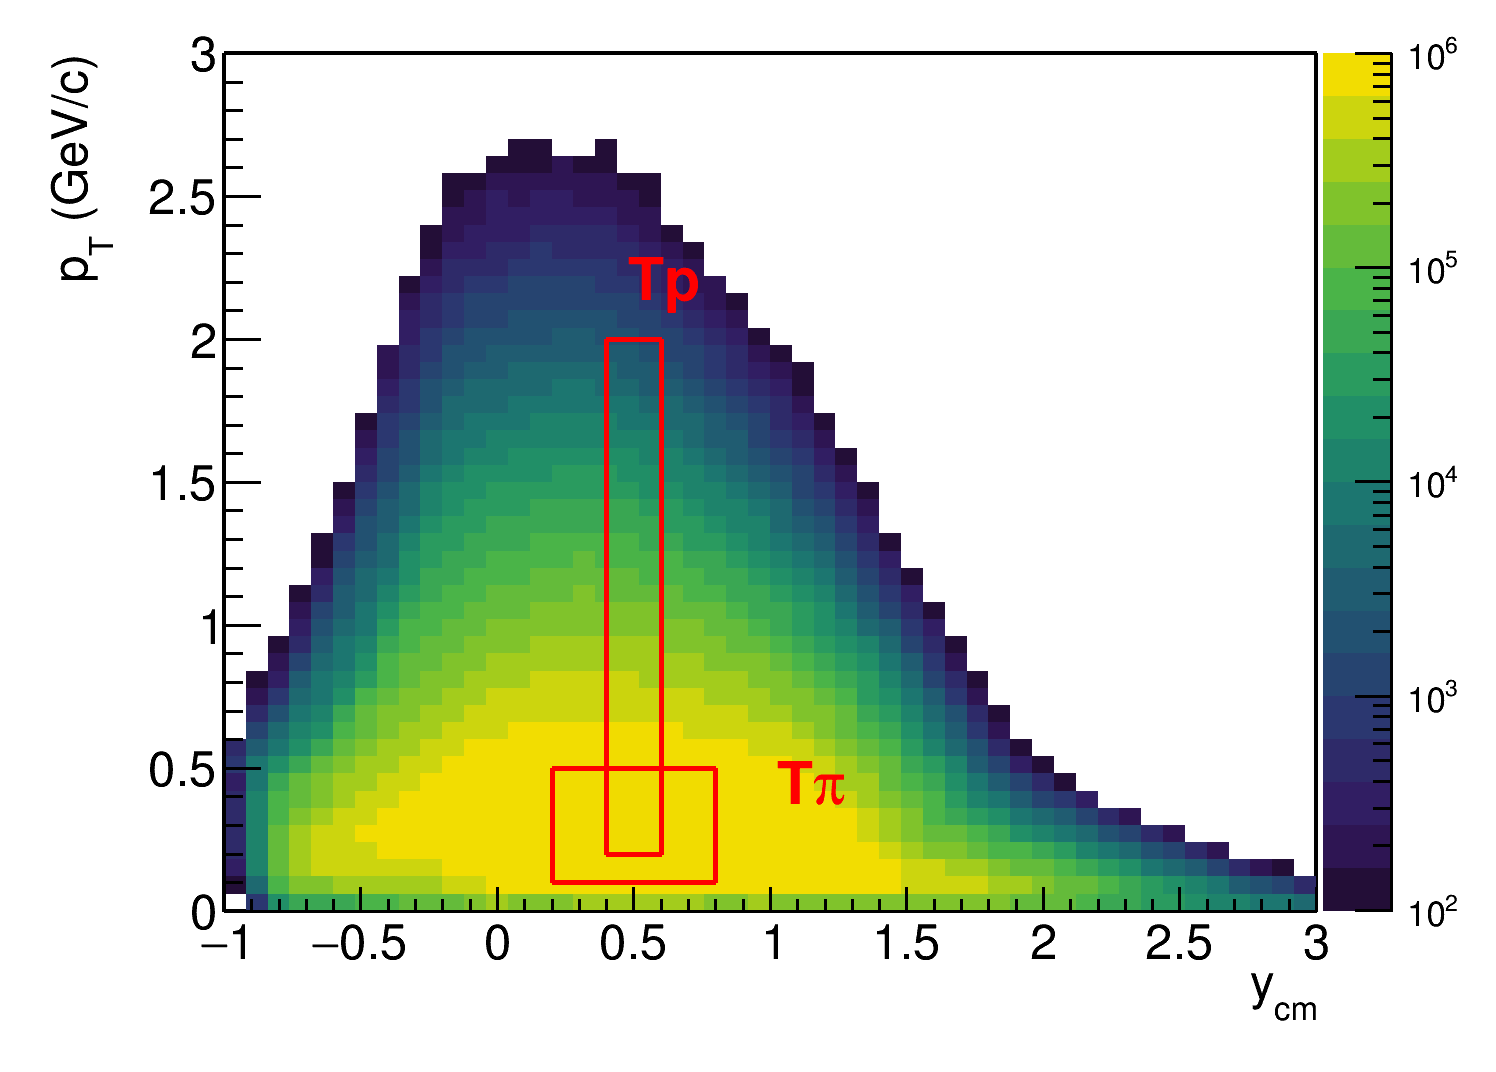
\includegraphics[width=0.38\linewidth]{images/pT_ycm_protons.png}
\caption{
Слева: Схема разделения модулей FCHal по группам для определения плоскости симметрии события.
Справа: Кинематические окна для подсчета $Q_1$-векторов из треков заряженных частиц.
}
\label{fig:bmn_subevents}
\end{center}
\end{figure}

\begin{figure}[h]
  \begin{center}
  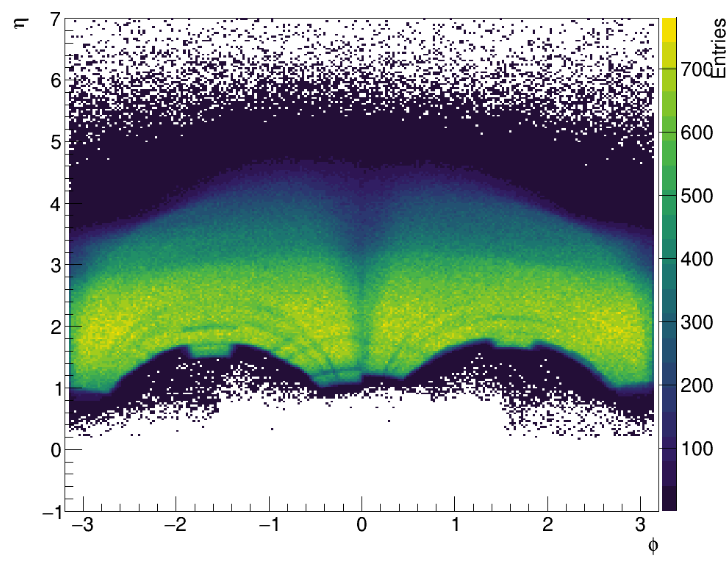
\includegraphics[width=0.45\linewidth]{images/bmn_phi_eta.png}
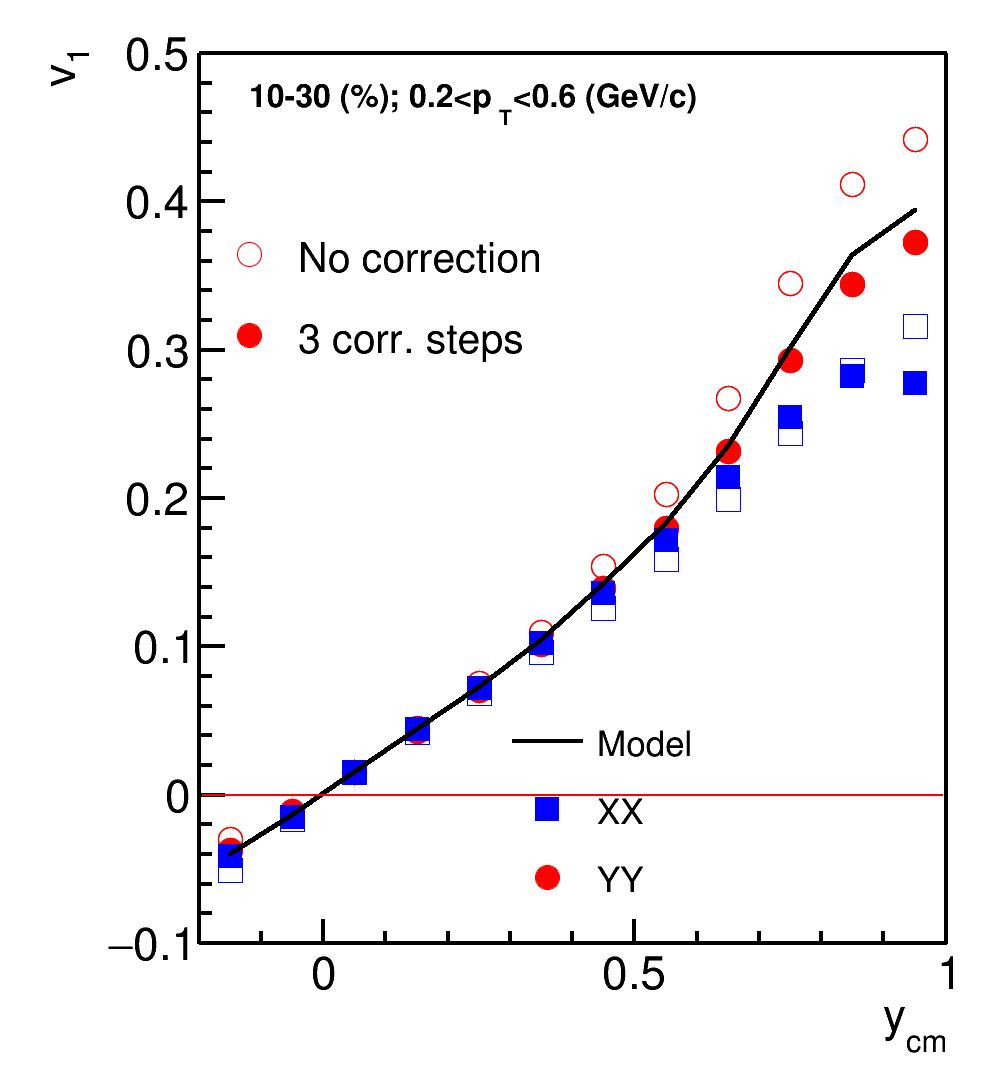
\includegraphics[width=0.33\linewidth]{images/v1_proton_correction_rapidity.png}
\caption{Азимутальный аксептанс трековой системы BM@N (слева). Сравнение  $v_1(y_{cm})$ протонов в  модельных столкновениях Xe+Cs(I) 
  для различных компонент $u_1$-вектора (справа) до и после коррекции на азимутальную
  неоднородность аксептанса детектора. }
\label{fig:bmn_components}
\end{center}
\end{figure}

Азимутальный аксептанс трековой системы BM@N сильно неоднороден (см. рис.~\ref{fig:bmn_components} (слева)).
Результат  применения коррекций на азимутальную неоднородность представлен на рис.~\ref{fig:bmn_components} (справа).
Разными цветами обозначены значения $v_1(y_{cm})$ протонов, полученные с использованием различных компонент $u_1$-вектора. 
Открытые и закрытые маркеры обозначают результаты до и после коррекции, соответственно.
Линией обозначены значения $v_1$  извлеченные напрямую из модели JAM.
После применения 3 ступеней коррекции, результаты полученные при помощи $YY$ корреляции $u_1$ и $Q_1$-векторов, хорошо согласуются с результатами из модели.
Напротив, значения $v_1$, посчитанные с использованием $XX$-компонент, расходятся с модельными  $v_1$. 
Причиной может служить сильное отклонение частиц в направлении оси $x$ в магнитном поле. 
В связи с этим, в дальнейшем для анализа могут быть использованы лишь корреляции $YY$-компонент $u_1$ и $Q_1$-векторов.
На рис.~\ref{fig:bmn_combinations} представлена зависимость разрешения плоскостей симметрии F1, F2 и F3 от центральности для различных комбинаций $Q_1$-векторов.
Значения $R_1$, полученные при помощи разделенных по быстроте комбинаций, согласуются между собой в пределах статистической ошибки для всех трех плоскостей симметрии. 
Значительное отличие значений $R_1$, полученных с использованием комбинаций не разделенных по быстроте $Q_1$-векторов, может быть объяснено распространением адронного ливня в поперечном направлении, что вызывает дополнительные корреляции между векторами $F1$ и $F2$, и $F1$ и $F3$~\cite{Mamaev:2023fpr}.
%
\begin{figure}[h]
\begin{center}
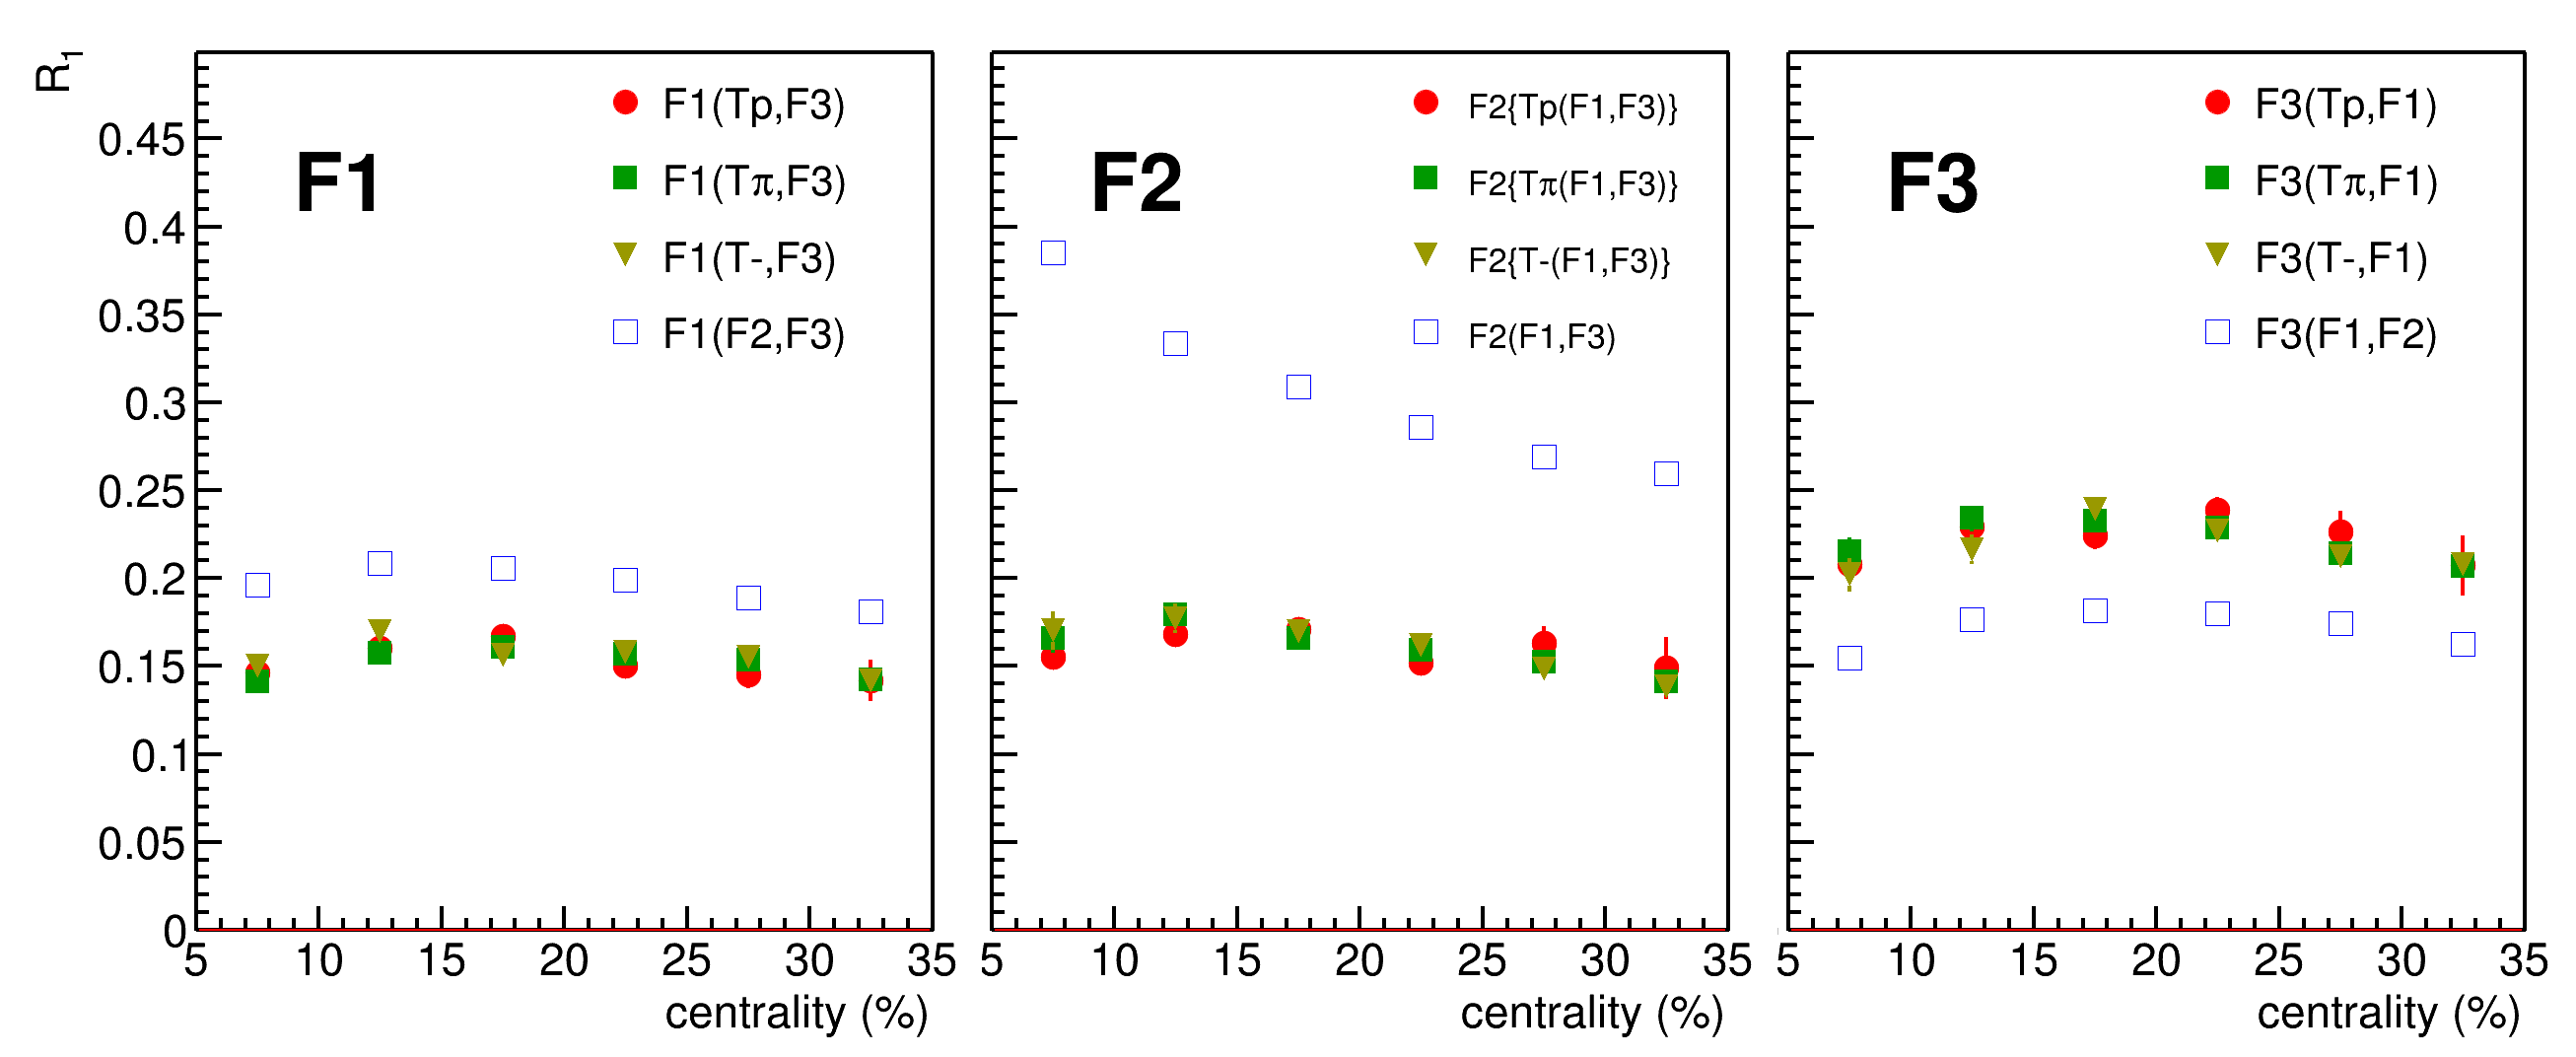
\includegraphics[width=0.87\linewidth]{images/R1_F123_combinations_centrality.png}
\caption{Зависимость разрешения плоскостей симметрии F1-F3 от центральности для различных комбинаций $Q_1$-векторов, см. текст.}
\label{fig:bmn_combinations}
\end{center}
\end{figure}

На рисунке~\ref{fig:bmn_v1_v2} показаны результаты сранения значений  $v_1$($y_{cm}$) (слева) и $v_2$($p_{T}$) (справа) полученных  из анализа полностью реконструированных в BM@N протонов (маркеры) и 
модельных данных (линии) для Xe+Cs(I) столкновений при энергиях 2 - 4 АГэВ~\cite{Mamaev:2023yhz,Mamaev:2024}. 
Разными цветами обозначена разная энергия столкновений. 
Между данными извлеченными из модели и результатами анализа после реалистичной цепочки реконструкции наблюдается согласие в пределах статистических ошибок. 
%
\begin{figure}[h]
\begin{center}
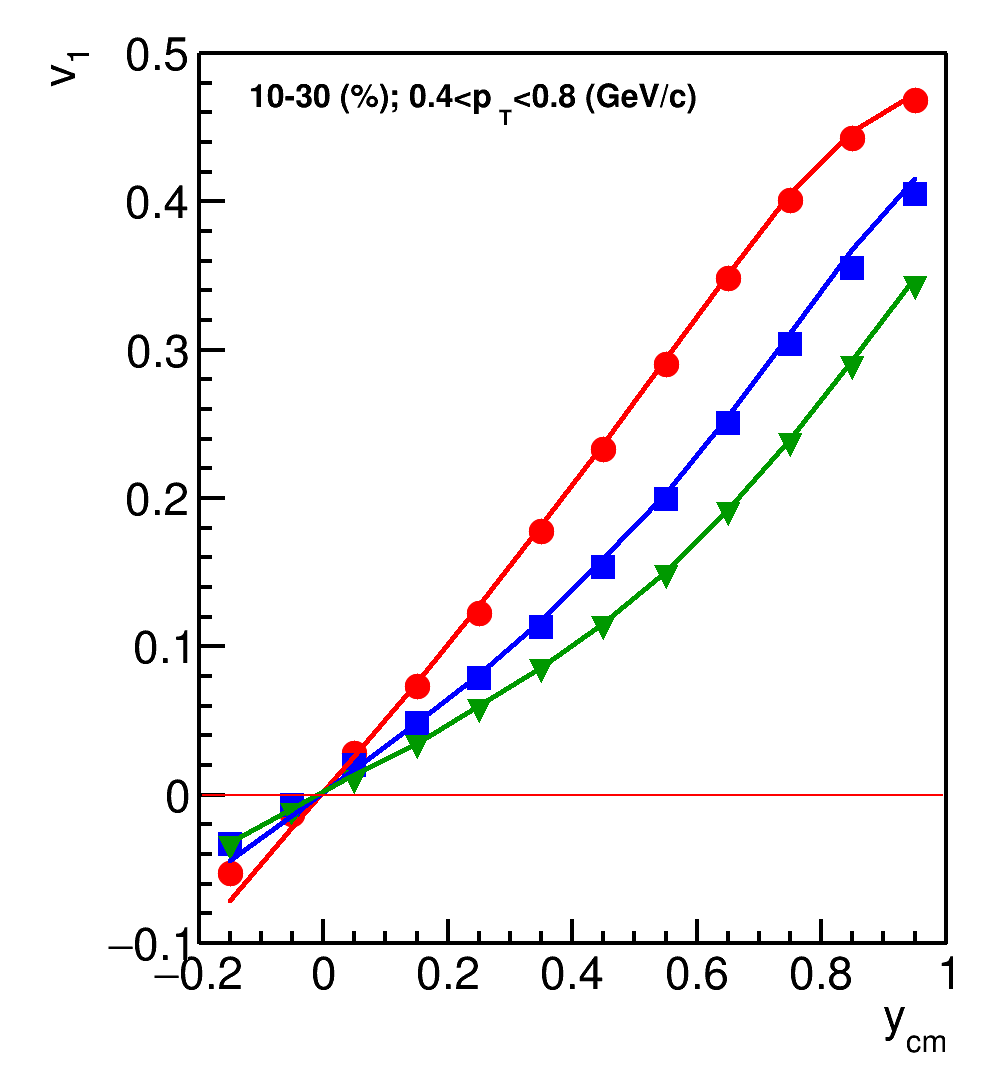
\includegraphics[width=0.4\linewidth]{images/v1_proton_tof_rapidity.png}
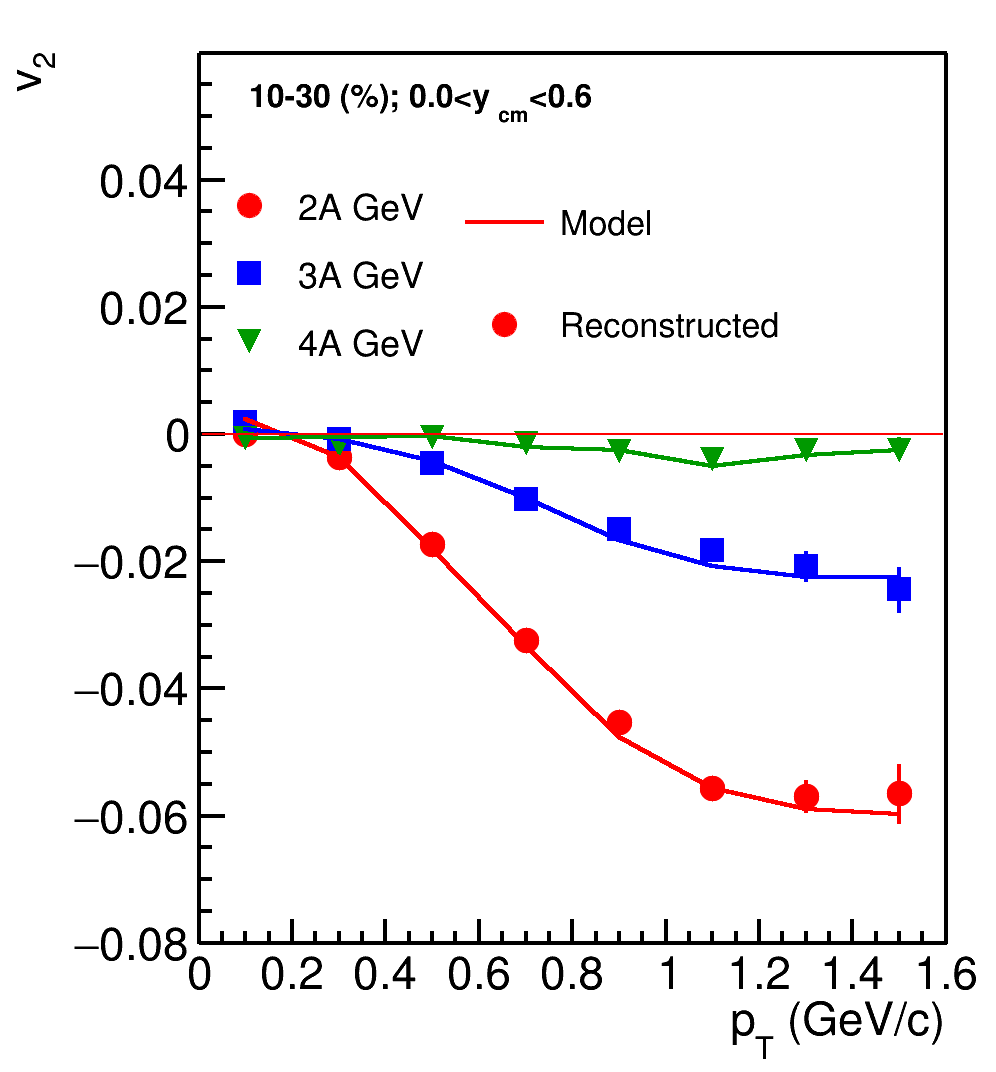
\includegraphics[width=0.4\linewidth]{images/v2_proton_tof_pT.png}
\caption{Cравнение  $v_1$($y_{cm}$) (слева) и $v_2$($p_{T}$) (справа) из анализа полностью реконструированных в BM@N протонов (маркеры) и 
модельных данных (линии) для Xe+Cs(I) столкновений при энергиях 2 - 4 АГэВ. }
\label{fig:bmn_v1_v2}
\end{center}
\end{figure}

В \underline{\textbf{заключении}} приведены основные результаты работы, которые заключаются в следующем:
%% Согласно ГОСТ Р 7.0.11-2011:
%% 5.3.3 В заключении диссертации излагают итоги выполненного исследования, рекомендации, перспективы дальнейшей разработки темы.
%% 9.2.3 В заключении автореферата диссертации излагают итоги данного исследования, рекомендации и перспективы дальнейшей разработки темы.
\begin{enumerate}
  \item Разработан метод учета корреляций не связанных с коллективным
движением рожденных частиц (непотоковых корреляций) и изучено
их влияние на результаты измерения коллективных потоков в области энергий 1.2-4 АГэВ. 
  \item Впервые получены зависимости  $v_1$ протонов от быстроты и поперечного импульса, а так же наклона $dv_1/dy_{cm}|_{y_{cm}}$ в 
  области средних быстрот в столкновениях \au{} при  энергии  $E_{kin}=$1.23$A$~ГэВ и \ag{} 
  при энергиях $E_{kin}=$1.23$A$ и $E_{kin}=$1.58$A$~ГэВ в эксперименте HADES. Полу­ченные новые результаты измерения $v_1$ протонов современными методами 
  анализа являются принципиально важными для проверки и
дальнейшего развития теоретических моделей ядро-ядерных столкновений.
  \item Обнаружено масштабирование направленного потока протонов с временем пролета ядер $t_{pass}$ и геометрией столкновения в области
   энергий $E_{kin}=$1.23$A$ и $E_{kin}=$1.58$A$~ГэВ, что позволяет оценить влияние спектаторов налетающего ядра на
формирование направленного потока протонов.
  \item На основе моделирования установки детально изучены возможности измерения коллективных потоков протонов на экспериментальной установке BM@N на ускорителе
NUCLOTRON-NICA (ОИЯИ, Дубна). Это позволо расширить существующую физическую программу эксперимента BM@N.
\end{enumerate}


%\newpage
% При использовании пакета \verb!biblatex! список публикаций автора по теме
% диссертации формируется в разделе <<\publications>>\ файла
% \verb!../common/characteristic.tex!  при помощи команды \verb!\nocite! 

\ifthenelse{\equal{\thebibliosel}{0}}{% Встроенная реализация с загрузкой файла через движок bibtex8
  \renewcommand{\refname}{\large \authorbibtitle}
  \nocite{*}
  \insertbiblioauthor                          % Подключаем Bib-базы
  %\insertbiblioother   % !!! bibtex не умеет работать с несколькими библиографиями !!!
}{% Реализация пакетом biblatex через движок biber
  \begin{refcontext}[labelprefix={A}]
    \insertbiblioauthor                          % Подключаем Bib-базы
  \end{refcontext}
  
  \begin{refcontext}[labelprefix={B}}]
    \insertbiblioother
  \end{refcontext}
}

% \end{linenumbers}
         % Содержание автореферата

\end{document}